%!TEX root = ../Document.tex

This chapter gives a compact review of the theoretical aspects and methods used in the presented study. For in-depth explanations please use the references provided.

\section{Materials Section}

\subsection{Laser Induced Graphene}

The effect of direct laser carbonization of the polymeric materials was first reported by Srinivasan \textit{$et\ al.$}  \cite{Srinivasan} in 1994, who found that ultraviolet laser irradiation of  polyimide PMDA-ODA (Kapton$^{TM}$) yields a patternable, porous, electrically conducting carbon network. Later in 2014 Tour's group has found similar effect for the polyimide (PI) Kapton$^{TM}$ surfaces treated by CO$_2$ laser in IR spectrum \cite{lin_laser-induced_2014}. The proposed chemical process is schematically shown in Figure \ref{fig:PI-into-graphene}. 


\begin{figure}[H]
\centering
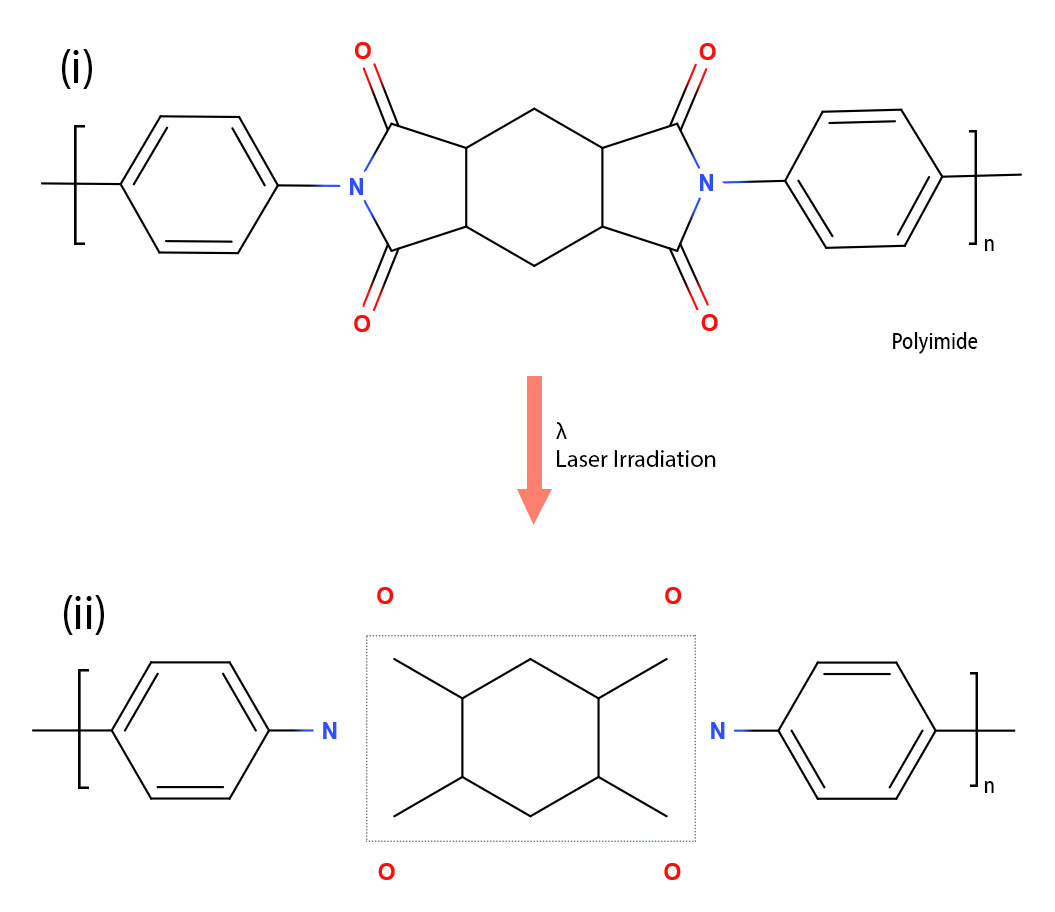
\includegraphics[width=0.9\textwidth]{Figures/Theory/Polyimide-into-graphene.jpg}
\medskip
\caption{Pyrolitic synthesis of laser-induced graphene (LIG). (i) Structure of polyimide film; (ii) Structural change of polyimide after laser irradiation}
\label{fig:PI-into-graphene}
\end{figure}

Figure \ref{fig:LIN-2015} sums up the procedure leading to LIG formation by irradiating a commercial PI film with a $CO_2$ infrared laser under ambient conditions.

\begin{figure}[H]
\centering
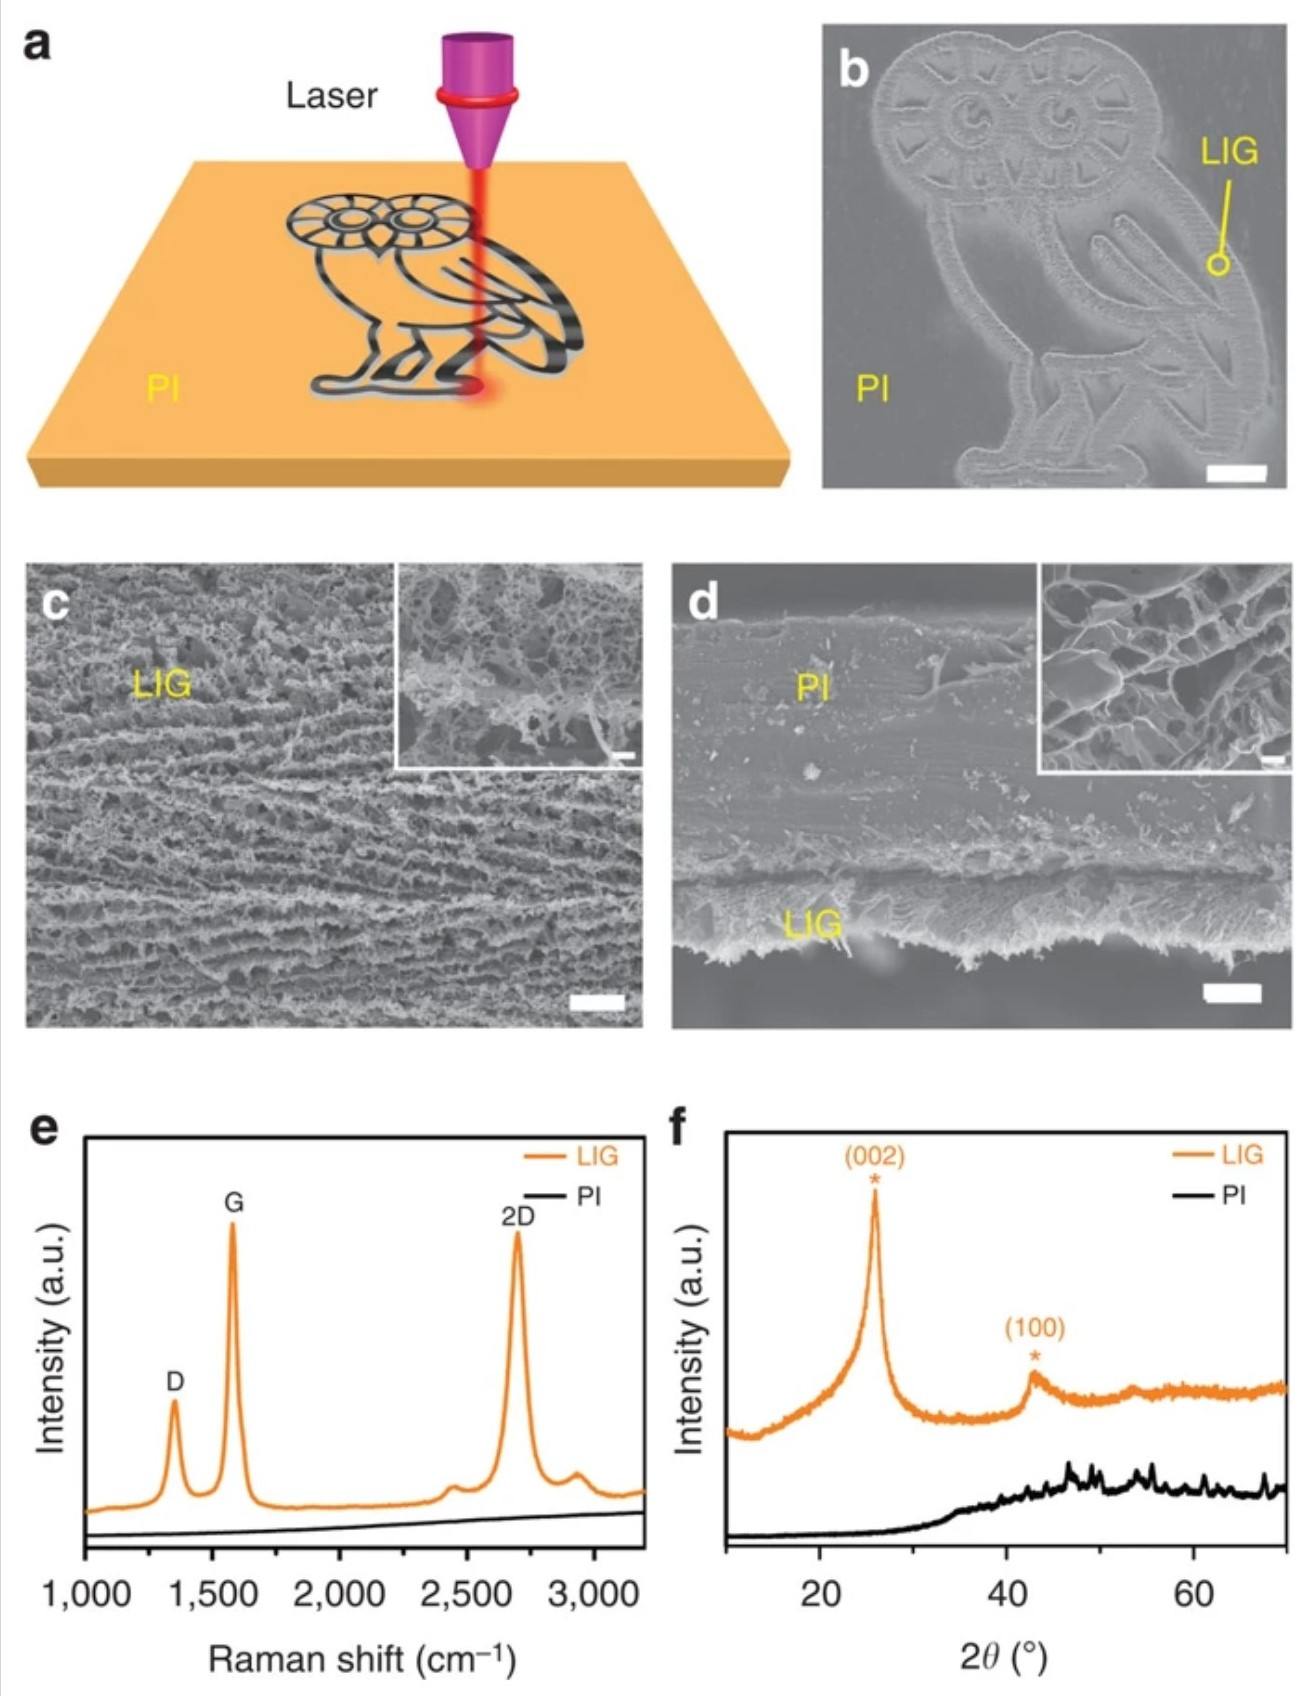
\includegraphics[width=1\textwidth]{Figures/Theory/LIN-2014.jpg}
\medskip
\caption{(a), Schematic of the synthesis process of LIG from PI. (b), SEM image of LIG patterned into an owl shape; scale bar, 1 mm. The bright contrast corresponds to LIG surrounded by the darker-colored insulating PI substrates. (c), SEM image of the LIG film circled in (b); scale bar, 10 $\mu$m. Inset is the corresponding higher magnification SEM image; scale bar, 1 $\mu$m. (d), Cross-sectional SEM image of the LIG film on the PI substrate; scale bar, 20 $\mu$m. Inset is the SEM image showing the porous morphology of LIG; scale bar, 1 $\mu$m. (e), Representative Raman spectrum of a LIG film and the starting PI film. (f), XRD of powdered LIG scraped from the PI film \cite{lin_laser-induced_2014}.}
\label{fig:LIN-2015}
\end{figure}

Changes in chemical structure of initial polyimide substrate have shown formation of the graphitic structures on the final product of laser pyrolysis which was demonstrated by characteristic Raman spectrum showing D and G lines for the final product as in Figure \ref{fig:LIN-2015}(e). Figure \ref{fig:LIG-FTIR_Lin} shows characteristic change of FTIR spectra of PI as compared to the obtained LIG.

\begin{figure}[H]
\centering
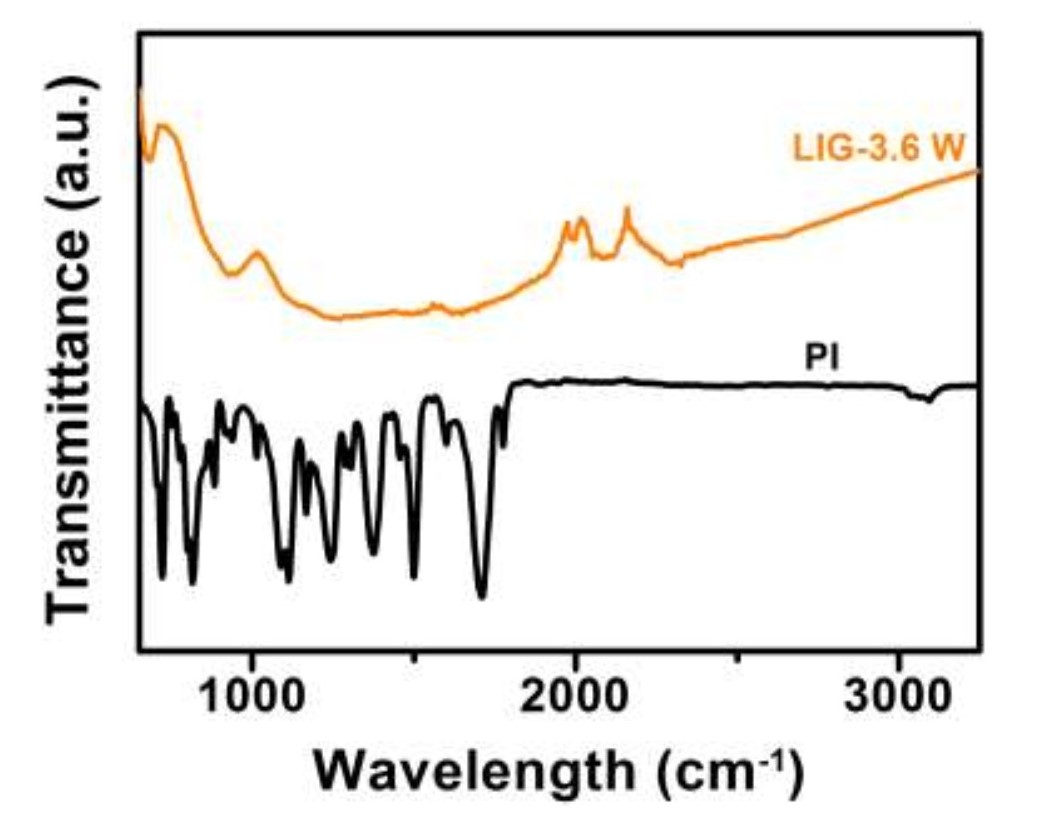
\includegraphics[width=0.5\textwidth]{Figures/Theory/FTIR_LIG_Lin.jpg}
\medskip
\caption{FTIR  spectra of LIG obtained at laser power of 3.6 W  and  PI  films. FTIR  spectra of PI showing distinct peaks  at  1090-1776 $cm^{-1}$, corresponding  to  the  well-defined  stretching  and bending modes of the C-O, C-N and C=C bonds. After the laser scribing, a broad absorption from 1000 $cm^{-1}$ to 1700 $cm^{-1}$ shows that the laser scribing leads to a large variation in the local environment \cite{lin_laser-induced_2014}.}
\label{fig:LIG-FTIR_Lin}
\end{figure}

\textbf{Formation and Morphology of LIG}

Short laser pulses enable a rapid heating of a precursor which causes laser induced pyrolysis taking place at temperatures over 900$\degree C$. The material prepared by the laser treatment of the polyimide films was shown to consist of graphene and is nowadays referenced as laser induced graphene, $i.e.$ LIG \cite{lin_laser-induced_2014}. 

On the atomic level LIG has a graphene structure of flat hexagonal carbon rings organized in infinite honeycomb crystal lattice as can be seen in Figure \ref{fig:real-graphene} \cite{Graphene}. Flat layers are further stacked into 3D structures well known as the graphite material \cite{katsnelson_2012}. 


\begin{figure}[H]
\centering
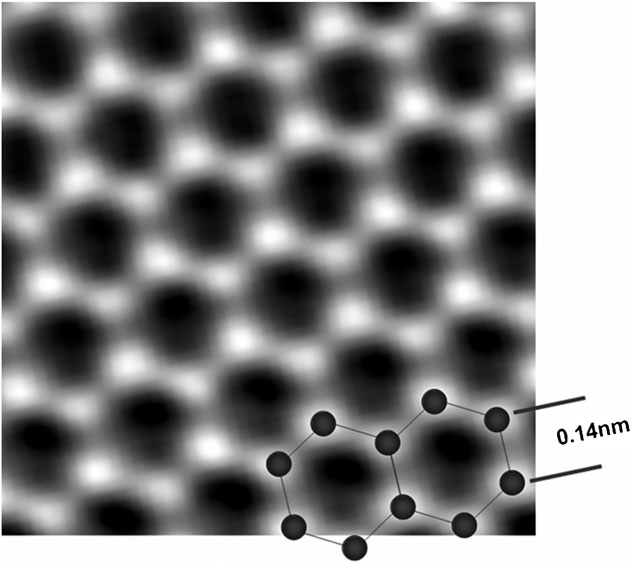
\includegraphics[width=0.5\textwidth]{Figures/Theory/Real_graphene.jpg}
\medskip
\caption{Graphene: image of graphene in TEM by Berkeley’s TEAM05 \cite{Graphene}.}
\label{fig:real-graphene}
\end{figure}

For the microstructure of LIG it was found that laser settings can drastically affect the final morphology. Tour \textit{$et\ al.$} investigations of LIG formation concluded that the minimum threshold for polyimide precursors to be transformed into conductive carbonaceous material lays at the laser fluence $H$ values of $\approx$ 5$\ J\cdot cm^{-2}$. The resultant LIG material has porous microstructure predominantly consisting of flat flocculent particles, hence its notation as flat or porous LIG. Further increase in laser power, $i.e.$ fluence values $H$ up to $>\ 40\ J\cdot cm^{-2}$, leads according to Tour to LIG-fibers which shows fibrous morphology constituted by ultrathin carbonaceous fibers \cite{DUY2018472}. 


\textbf{Electrical Properties of LIG}

Among other physical properties of LIG one of the greatest interest in this thesis is its electrical resistance $R$. 
Typically for compact organized materials ($i.e.$ without voids in bulk) the main two factors defining their electron conductivity are attributed to the lattice structure and crystalline defects present in bulk \cite{gross2012festkoerperphysik}. However it was shown that for graphene and graphite fragments organized into porous 3D structures, the conductive behavior is drastically affected by mechanical particle arrangement mechanisms as they play a major role defining particle contact area in the bulk \cite{marinho_electrical_2012}. In general it was found that LIG materials have high electrical conductivity (5-25 S/cm) \cite{doi:10.1002/adma.201803621}. 

One of the latest studies conducted at the Laboratory of Applied Materials for Printed and Soft (LAMPSe) in TU Graz has shown that the electrical properties of LIG are directly dependent on its morphology, namely that the flat LIG has lower electrical conductivity than the LIG-fiber \cite{david}. 

\textbf{LIG Porosity and Surface Area}

To date the  literature provides only sole case studies regarding the LIG porosity and its surface area. Most of the papers refer to the results of Lin \textit{$et\ al.$} 2014 \cite{lin_laser-induced_2014}. In this study the LIG was obtained from Kapton PI precursor (Cat. No. 2271K3, thickness: 0.005$\;$inch) at laser power of 3.6 W. By the means of Brunauer–Emmett–Teller analysis (BET) the specific surface area of the LIG was determined to be $\sim 342m^2/g$. It was shown that this LIG was a mesoporous material with the pore sizes distributed at 2.36 nm, 3.68 nm, 5.37 nm and 8.94 nm. In Figure \ref{fig:lin_BET} the differential pore volume distribution graph can be seen. 

\begin{figure}[H]
\centering
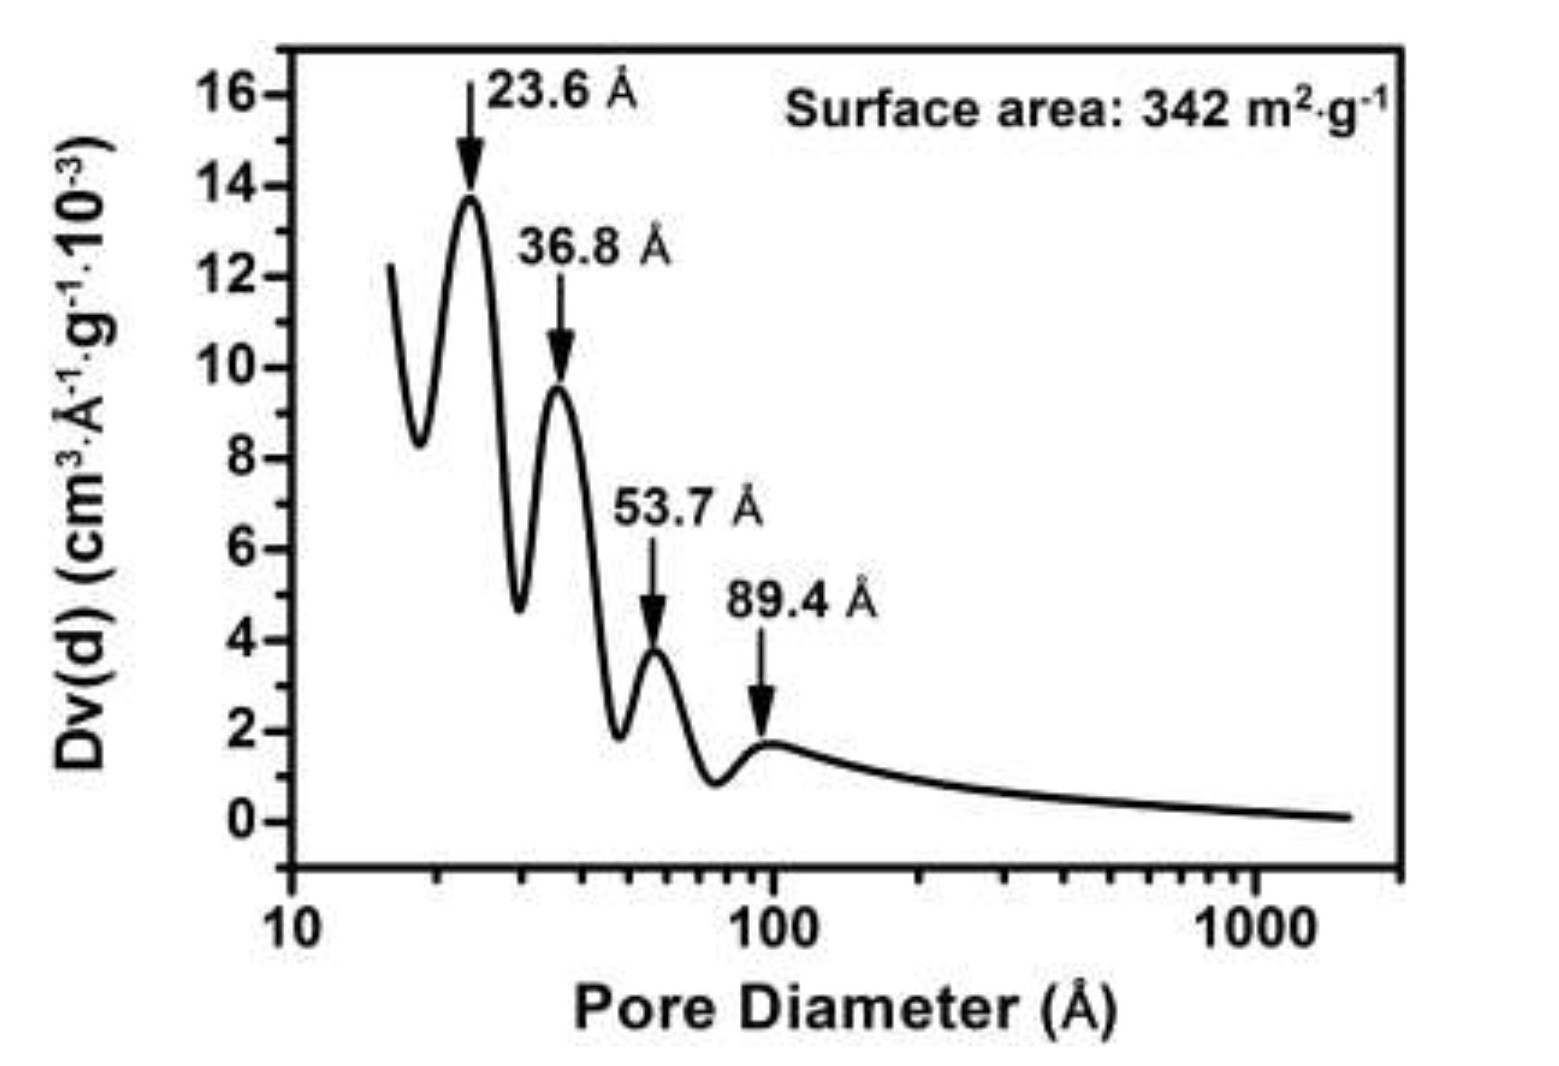
\includegraphics[width=0.6\textwidth]{Figures/Results/BET_results_LIN.jpg}
\medskip
\captionsetup{width=0.5\linewidth}
\caption{BET  specific  surface  area  of LIG-3.6  W from  \cite{lin_laser-induced_2014}}
\label{fig:lin_BET}
\end{figure}


\subsection{Elastic and Viscoelastic Biomaterials}

By IUPAC recommendations from 2012 the term biomaterial is defined as \textit{material exploited in contact with living tissues, organisms, or microorganisms}  \cite{TerminologyforbiorelatedpolymersandapplicationsIUPACRecommendations2012}. 

Within a big variety of biomaterials, two were used in this work and therefore their short introduction is presented in this subchapter.

\textbf{Polydimethylsiloxane (PDMS)} is a biocompatible \cite{wipff_covalent_2009}  structurally isotropic polymeric material with an empirical formula $CH_3[Si(CH_3)_2O]_nSi(CH_3)_3$, where n is the number of monomers repetitions. 


\begin{figure}[H]
\centering
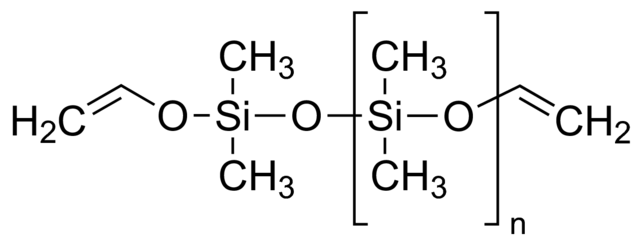
\includegraphics[width=0.5\textwidth]{Figures/Theory/PDMS-aldrich-large.png}
\medskip
\captionsetup{width=0.5\linewidth}
\caption{Structural formula of Polydimethylsiloxane (PDMS) \cite{PDMS_chem}}
\label{fig:PDMS-chem}
\end{figure}

A typical value of n is between 90 and 140 which leads to a molecular weight ranging from 6800 to 30000 g/mol. Depending on the length of the chain, the non-cross-linked PDMS may exhibit almost liquid (low n) or semi-solid (high n) properties. The siloxane bonds Si-C result in a flexible polymer chain with a high level of viscoelasticity. Further cross-linking of the chains into 3D network may be performed via addition or condensation mechanisms which lead to a hydrophobic elastomer \cite{ramli_cross-link_2011}. The final material is dielectric which is chemically inert, thermally  stable, permeable  to  gases \cite{prado_polydimethylsiloxane_2008}, transparent at optical frequencies (240 nM - 1100 nM) and exhibits isotropic and homogeneous mechanical properties \cite{wang_crosslinking_2014}.

As compared to other polymers thermal degradation process of cross-linked PDMS begins at relatively high temperatures around 350$\degree$C as can be seen from thermogravimetric analysis (TGA) in Figure \ref{fig:PDMS-thermo} \cite{camino_polydimethylsiloxane_2001}.

\begin{figure}[H]
\centering
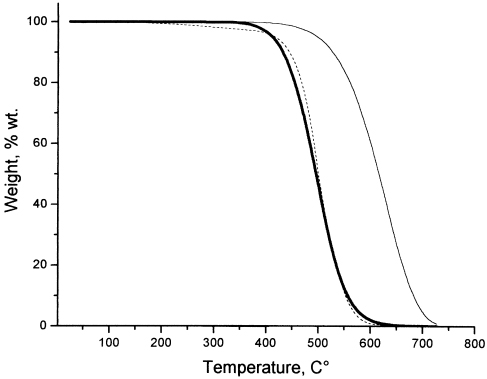
\includegraphics[width=0.6\textwidth]{Figures/Theory/PDMS-thermal-degradation.jpg}
\medskip
\captionsetup{width=0.7\linewidth}
\caption{TGA curves of PDMS (in N$_2$ atmosphere, at T rate of $10 \degree/min$). Experimental data: solid thick line; simulated: solid thin line \cite{camino_polydimethylsiloxane_2001}}
\label{fig:PDMS-thermo}
\end{figure}

As mentioned before PDMS shows high gas permeability for most of the common gas species including water vapor \cite{prado_polydimethylsiloxane_2008} as shown in Figure \ref{fig:PDMS_perm} from \cite{Metz}.

\begin{figure}[H]
\centering
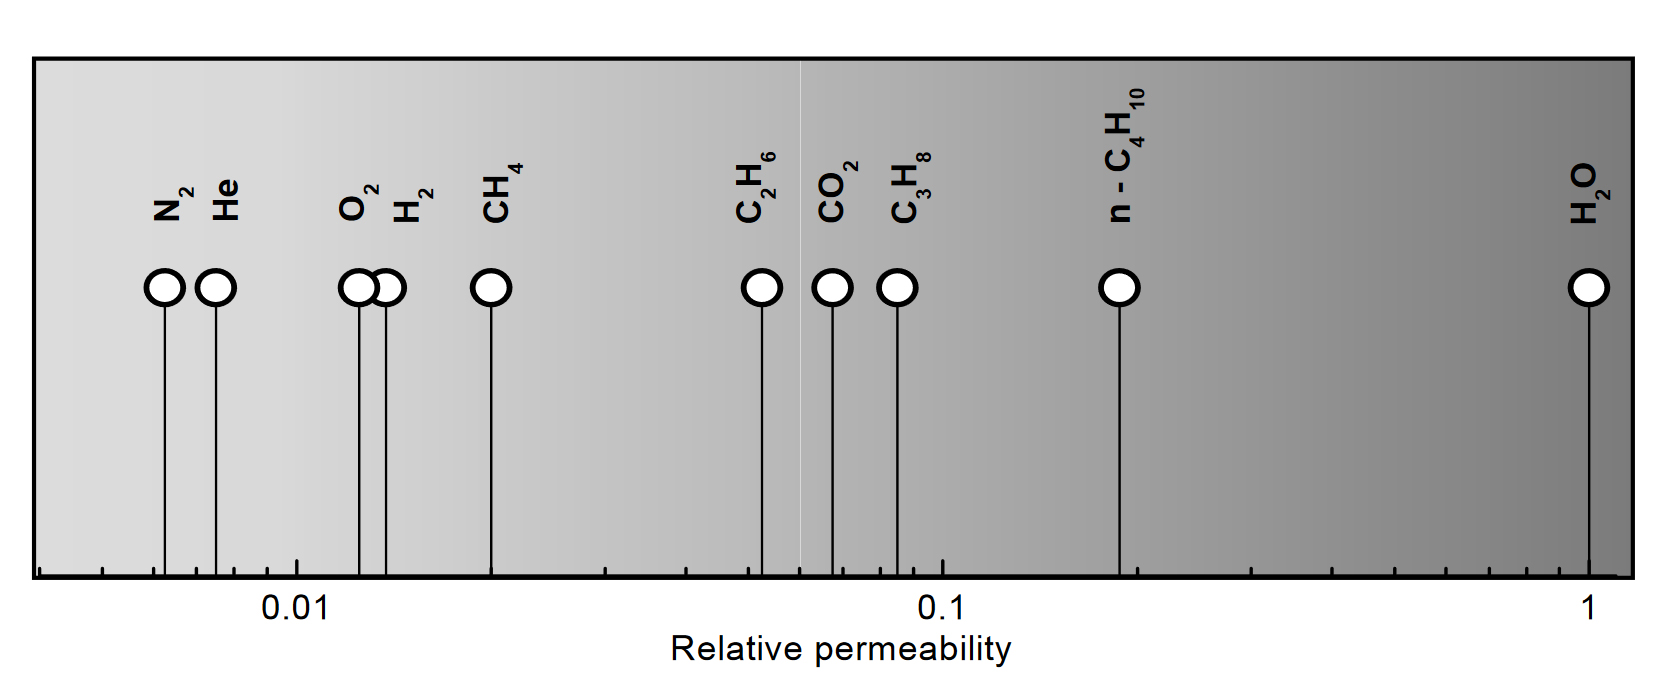
\includegraphics[width=1\textwidth]{Figures/Theory/PDMS-relative-permeability.jpg}
\medskip
\captionsetup{width=1\linewidth}
\caption{Relative  permeability  of  various  penetrants  compared  to  water vapor in  PDMS \cite{Metz}}
\label{fig:PDMS_perm}
\end{figure}


In absolute numbers water vapor permeation through PDMS reaches remarkably high value of 40000 $Barrer$. That fact is dictated by a small size of penetrant $H_2O$ molecules possessing low values of solubility and diffusivity even in a highly hydrophobic PDMS polymeric matrix \cite{Metz}. The permeation properties of selected gas species are listed in Table \ref{tab:PDMS_perm}.

\begin{table}[H]
\centering
    \caption[Caption for LOF]{Permeability Coefficients [Barrer]$^1$ for the PDMS \cite{prado_polydimethylsiloxane_2008}, \cite{Metz}}
    
    \label{tab:PDMS_perm} 
\medskip
\medskip
\begin{tabular}{ l | l | l | l | l | l} 

$N_2$ & $H_2$ & $O_2$ & $CH_4$ & $CO_2$ & $H_2O$ \\[15px]
\hline

 400 $\pm$ 10 &  890$\pm$30 & 800$\pm$20 & 1200$\pm$40 & 3800$\pm$70 &  40000$\pm$800                            \\[15px]


\end{tabular}
\\[15px]
\small\textsuperscript{1} 1 Barrer = $3.35\times 10^{-16} \frac{mol \times m}{m^2 \times s \times Pa}$\\
\end{table}
%

PDMS mechanical strength and Young's Modulus $E$ are dependant on cross-linking density \cite{wang_crosslinking_2014}. Zhixin Wang \textit{$et\ al.$} investigated this dependence for PDMS networks prepared from two component mixtures from Sylgard$^{TM}$ 184 silicone elastomer base and Sylgard$^{TM}$  184 silicone elastomer curing agent manufactured by Dow Corning (Mid-land, MI). The amount of curing agent used lays in direct correlation with the degree of cross-linking in the final elastomer. Greater cross-linking density leads to the higher stiffness of PDMS as can be seen from Figure \ref{fig:PDMS-mechan}. 

\begin{figure}[H]
\centering
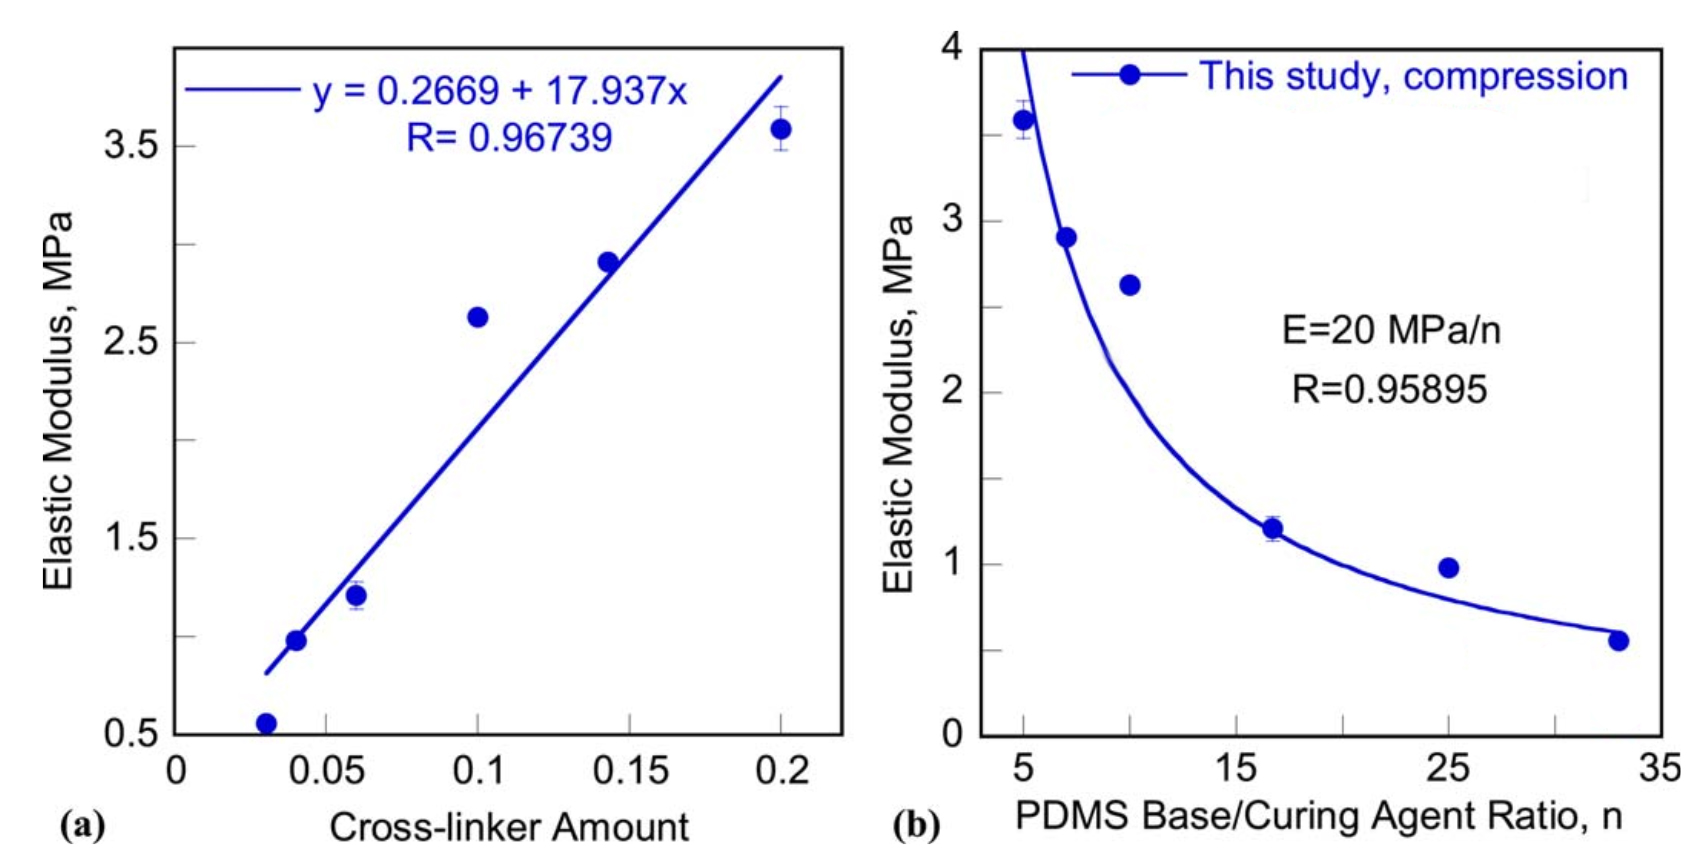
\includegraphics[width=1\textwidth]{Figures/Theory/PDMS-elastic-modulus.jpg}
\medskip
\captionsetup{width=1\linewidth}
\caption{(a) PDMS elastic modulus as a function of the curing cross-linker amount; (b) PDMS network elastic modulus \textit{vs.} PDMS Base/Curing agent weight ratio $n$ \cite{wang_crosslinking_2014}.}
\label{fig:PDMS-mechan}
\end{figure}

Elastic Modulus $E$ varies in the range of 0.5 - 3.5 MPa and can be in general approximated by an expression:

\begin{equation}
    E = \frac{20}{n}\ mPa
    \label{eq:young-pdms}
\end{equation}
 Where $n$ is the weight ratio of PDMS base to curing agent. 


Described properties make PDMS highly attractive for the fabrication of composite microstructures with implementation in biomedical systems \cite{mata_characterization_2005}, wearable applications and the internet of things. In these applications PDMS can play a role of a mechanically and chemically stable substrate or a sealed capsule carrying an electrical device.


\textbf{Polyurethane Medical Films}

Polyurethanes (PUs) are known to be extremely biocompatible materials \cite{SASTRI2014121}. PU chemical structure constitutes three complex monomers: a diisocyanate, a macrodiol, and a chain extender, variations of which lead to a number of different PU materials that can be synthesized \cite{KOHLI2019125}.

\begin{figure}[H]
\centering
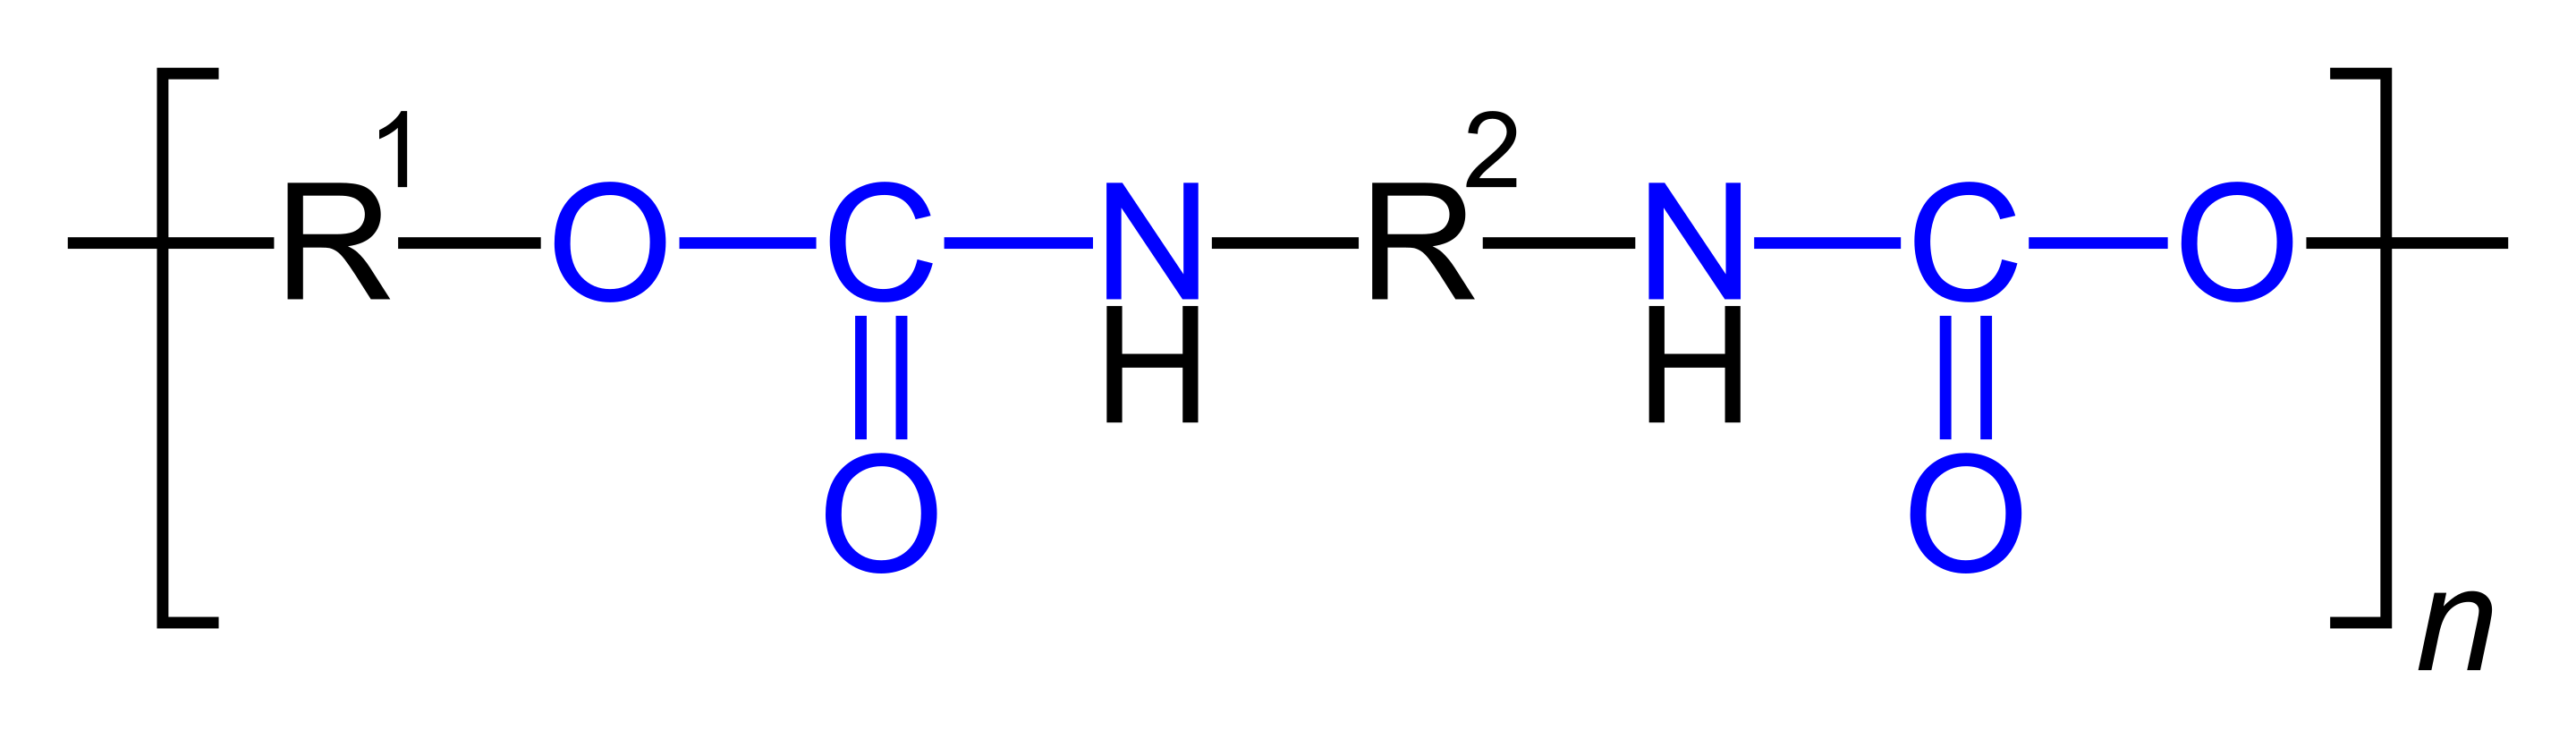
\includegraphics[width=0.6\textwidth]{Figures/Theory/2880px-Polyurethane-allg.png}
\medskip
\captionsetup{width=0.6\linewidth}
\caption{General structure of linear polyurethanes. The urethane groups are marked in blue. $R^1$ stands for the “rest” of the diol used for the synthesis (HO - $R^1$ - OH), $R^2$ stands for the “rest” of the diisocyanate (OCN - $R^1$ - NCO) \cite{Polyurethanen}.}
\label{fig:PU-structure}
\end{figure}

Polyurethanes can be produced in a form of ultrathin $\approx$20-40 $\mu$m highly viscoelastic transparent non-conductive films \cite{Fixomull}, which due to their high water vapor permeability and biocompatibility properties are widely used in medical applications as skin care. As it will be seen in the following chapters these properties of PU can be utilised for packaging when preparing flexible electrical devices such as thin supercapacitor cells. 


\subsection{Elastic Conductive Composites}

One of the objectives of this thesis was to study the possibility of creating an electrically conductive elastic composite  $\approx 100\mu m$ film based on LIG. The expected material was meant to be used for electrodes in flexible ionic supercapacitors and therefore additional goal was to find an optimal composition for storing high amounts of ionic charges. In this regard, we present a short review of the suitable for our goals LIG composite materials known to date.

So far a few groups reported creation of composite based on elastomeric substrate embedding LIG \cite{dallinger_stretchable_2020}, \cite{jeong_flexible_2019}, \cite{parmeggiani_pdmspolyimide_2019}, \cite{lamberti_highly_2016}.

\textbf{Jeong $et\; al.$ \cite{jeong_flexible_2019} group} created a strain sensor by placing a PI film on the prefabricated PDMS film of 400 $\mu m$ and irradiating the sandwich with an UV 355 nm pulsed laser. In this manner the desired graphitic pattern was implanted directly into the PDMS substrate. The remaining polyimide film was removed, leaving LIG pattern on the PDMS. The structure was then covered with another layer of PDMS to protect the pattern. Schematics of the procedure are presented in Figure \ref{fig:strain_jeong}. 


\begin{figure}[H]
\centering
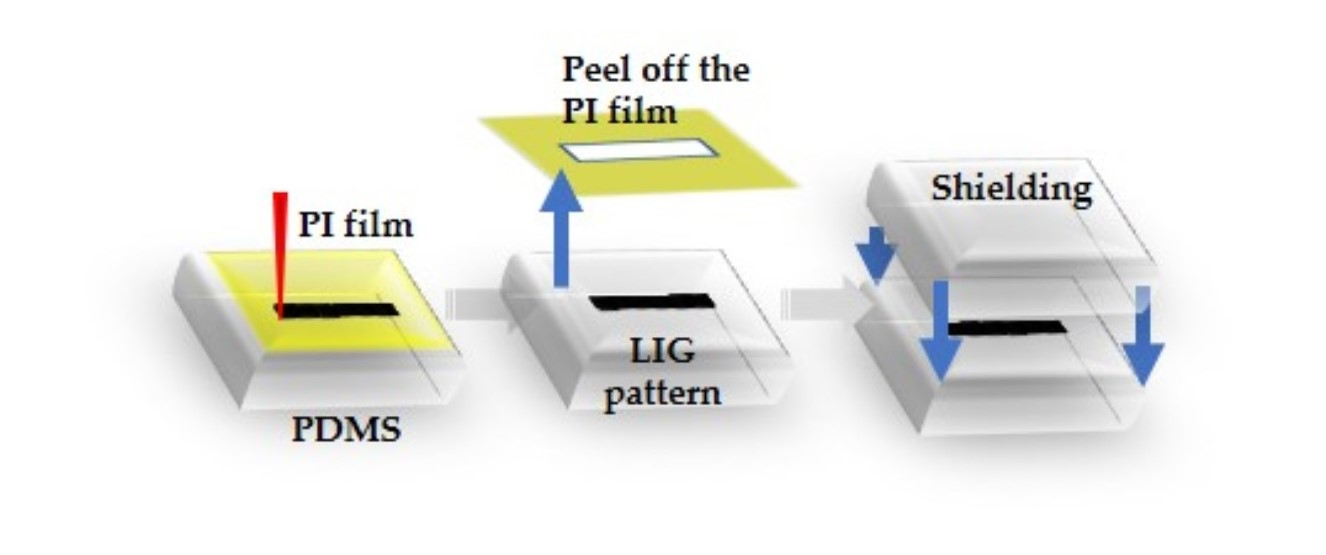
\includegraphics[width=0.8\textwidth]{Figures/Theory/Jeong.jpg}
\medskip
\captionsetup{width=0.8\linewidth}
\caption{Process of fabricating the LIG strain sensor \cite{jeong_flexible_2019}.}
\label{fig:strain_jeong}
\end{figure}

This method allowed the fabrication of sensitive and flexible piezoresistive type strain sensors in simple two steps. It was found to have a response time of $\approx$ 70 ms, good linearity to tensile strain, high gauge factors responsive to bending, and a low degree of creep in the bending/release cycle. 


\begin{figure}[H]
\centering
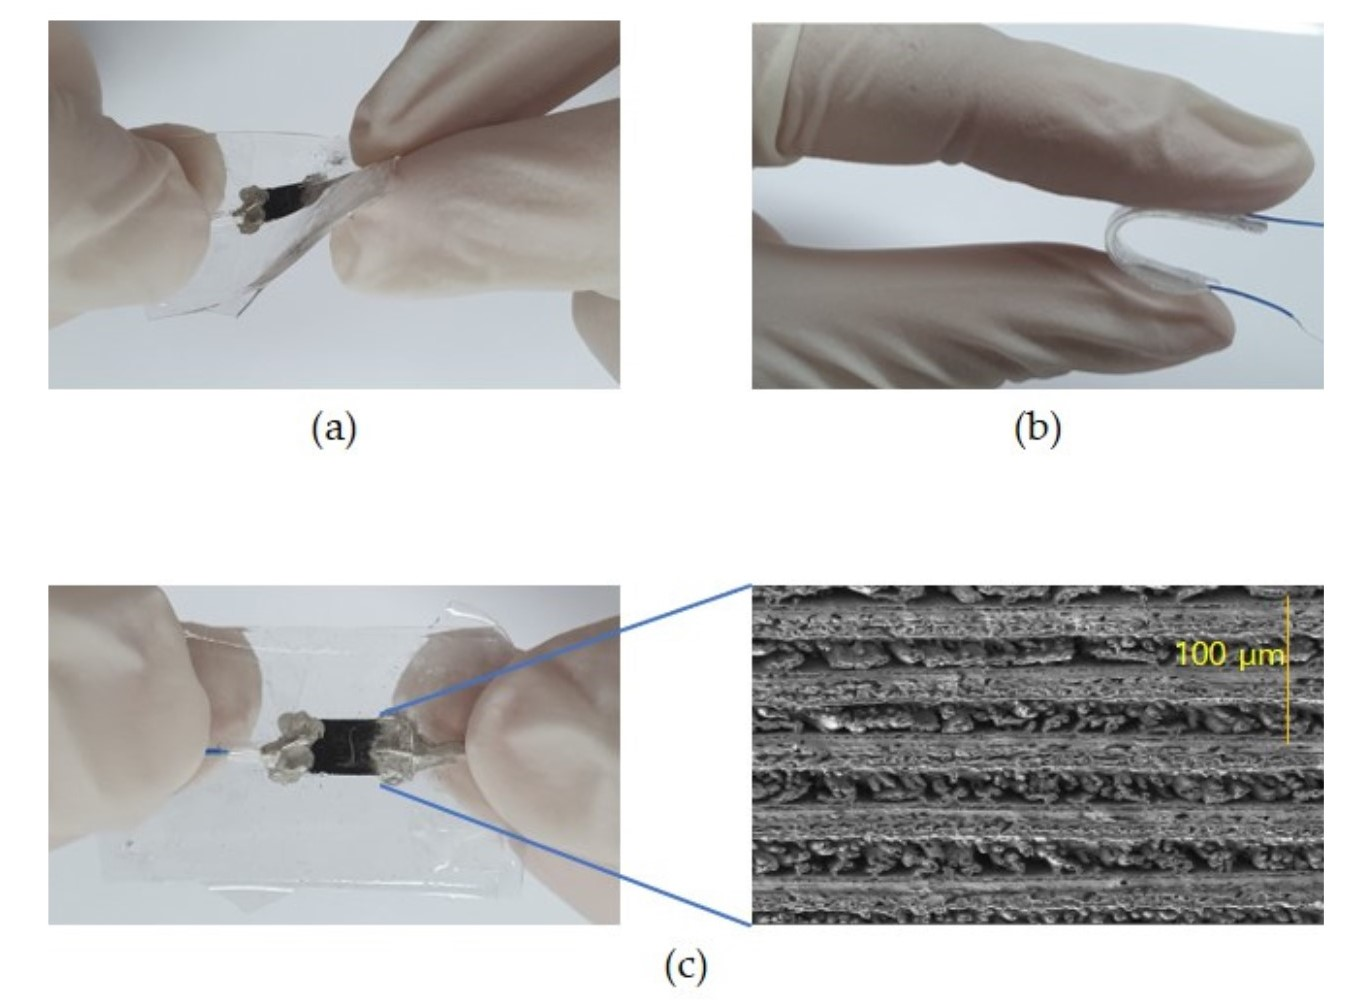
\includegraphics[width=0.7\textwidth]{Figures/Theory/Jeong_2.jpg}
\medskip
\captionsetup{width=0.9\linewidth}
\caption{Photographs of the strain sensor under (a) twisting and (b) bending;  (c) SEM image of carbonized pattern embedded on PDMS \cite{jeong_flexible_2019}.}
\label{fig:strain_jeong_2}
\end{figure}

\begin{figure}[H]
\centering
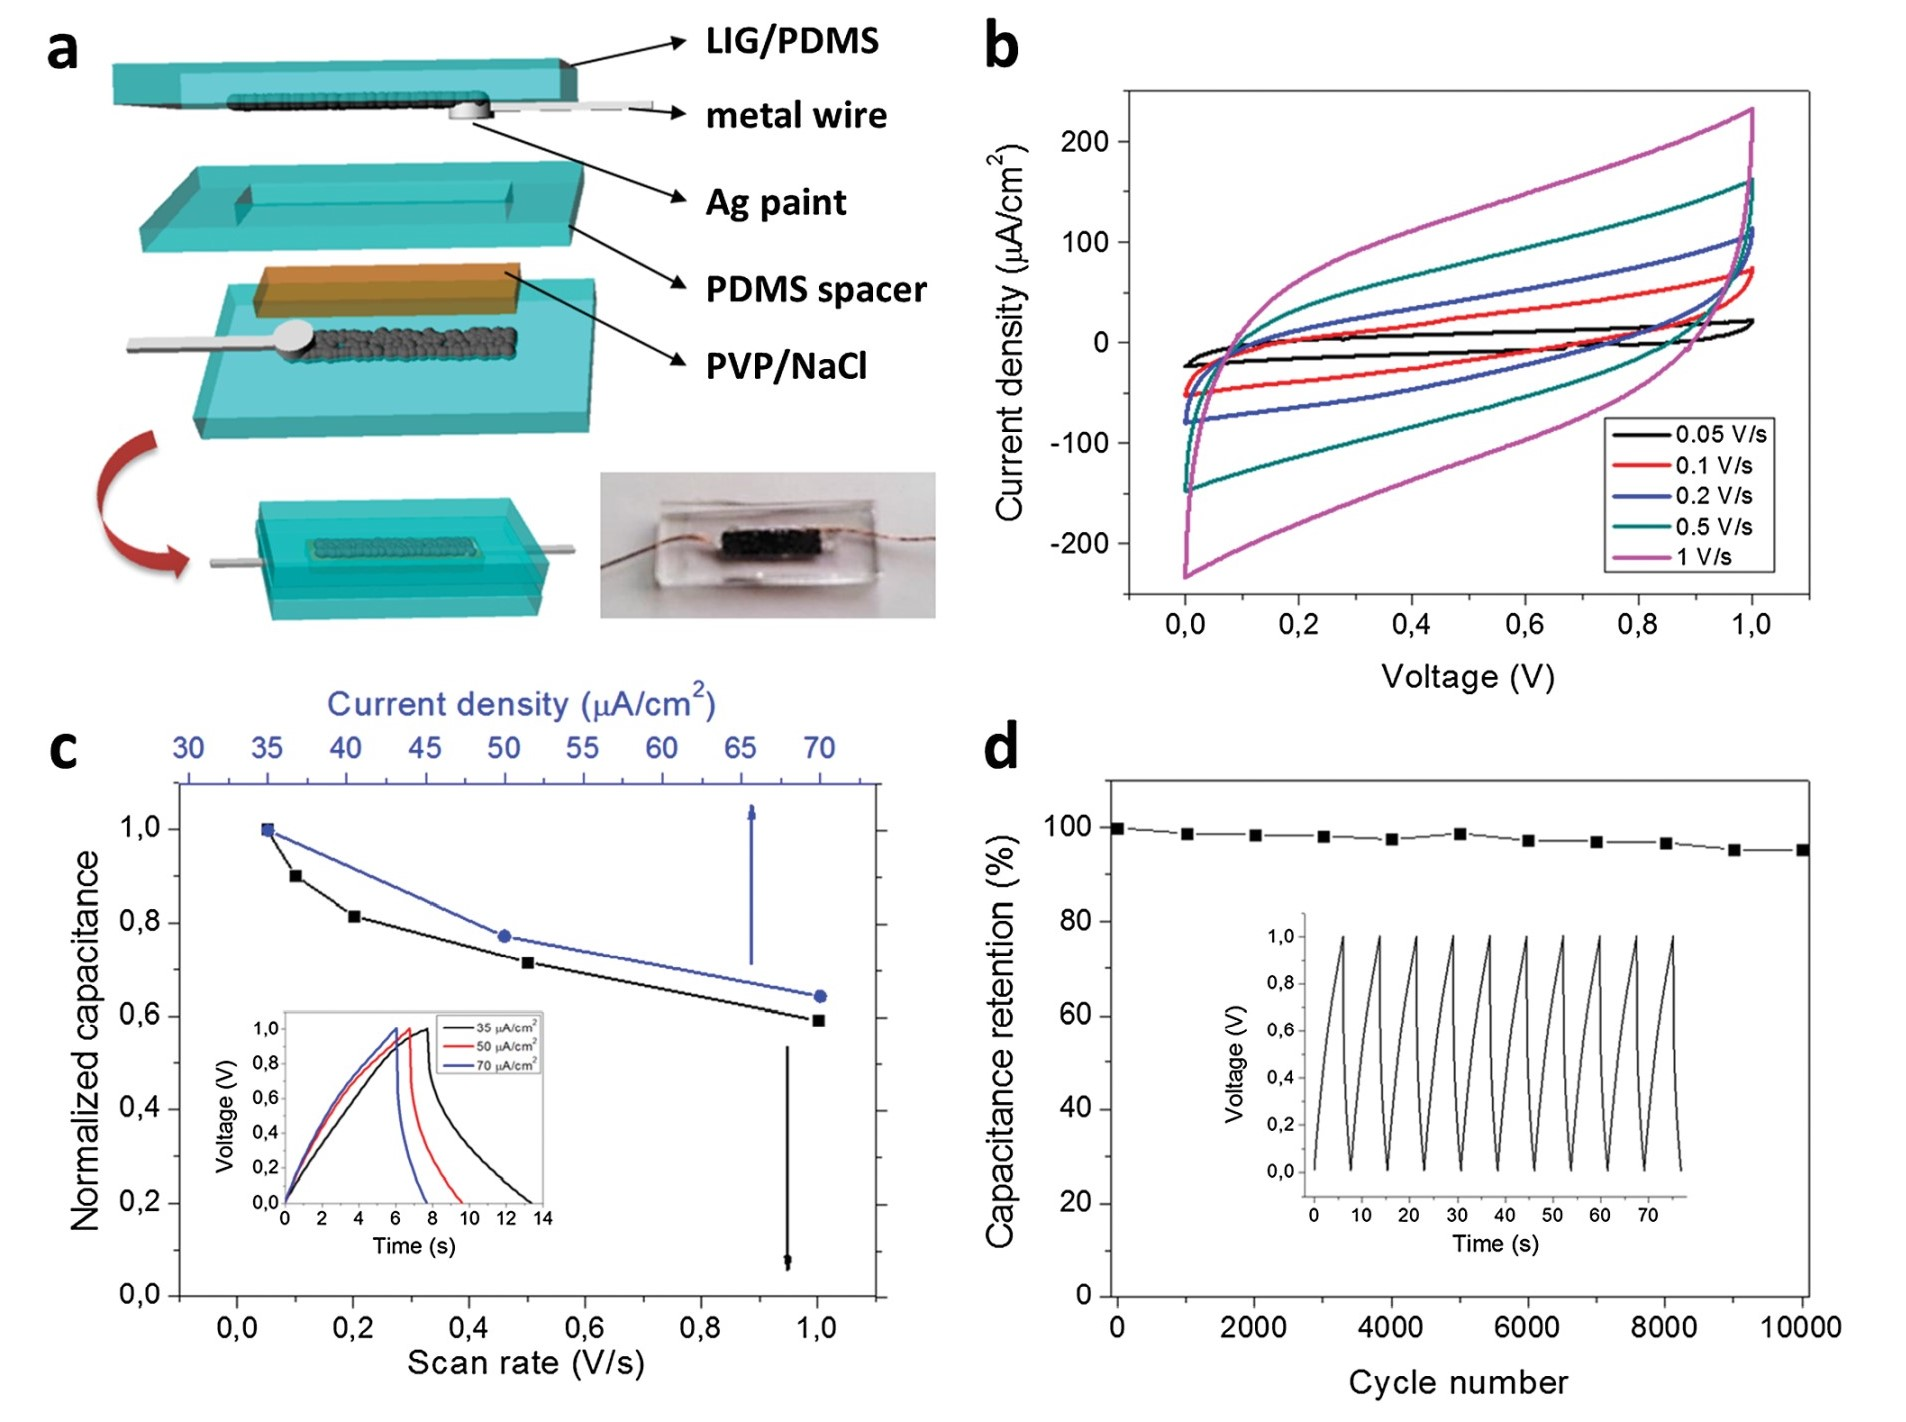
\includegraphics[width=0.95\textwidth]{Figures/Theory/Lamberti_PDMS_LIG_2016.jpg}
\medskip
\captionsetup{width=0.9\linewidth}
\caption{3D scheme of a) the LIG/PDMS supercapacitor assembly, in the inset a digital photograph of the assembled device is reported. Electrical characterization: b) CV at different scan-rates, c) capacitance trend $vs.$ scan rate and d) capacitance retention. The insets in (c) and (d) show the charge discharge profiles at different current and the cycling behavior at 70 $\mu A/cm^2$, respectively \cite{lamberti_highly_2016}.}
\label{fig:LIG_PDMS_Lamberti_2016}
\end{figure}

In 2016 \textbf{Lamberti $et \; al.$ \cite{lamberti_highly_2016} group} described a method to obtain a composite of LIG embedded into PDMS matrix. For that a porous LIG pattern was at first laser-scribed on a polyimide sheet using a nanosecond $CO_2$ laser; afterwards the PDMS mixture (Sylgard 184, Dow Corning, mixing ratio 15:1) was poured onto the conductive graphene circuit, the air bubbles were evacuated under vacuum; after that the PDMS was cured for 1 h at at 80 $\deg C$ and the LIG/PDMS composite sample was manually peeled off from PI substrate. According to the authors, obtained in this manner composite material showed mechanical properties typical of elastomers and at the same time had good electrical conductivity and high surface area. Two layers of the composite were used to prepare symmetrical planar electrochemical double layer (ECDL) supercapacitor cells filled with a Polyvinylpyrrolidone (PVP) gel with 1 M NaCl as shown in Figure \ref{fig:LIG_PDMS_Lamberti_2016}. From cyclic voltammetry (CV) curves obtained at scan rate of 50 $mV/s$ the maximum areal capacitance was calculated to be 650 $\mu F/cm^2$. 
 
\textbf{Lamberti $et \; al.$ \cite{parmeggiani_pdmspolyimide_2019} group} reported another approach for LIG PDMS composite formation where polyimide powder was firstly dispersed into a liquid PDMS mixture (in different concentrations, namely, 10, 25, 50, and 100 wt\% ) followed by cross-linking process to let PDMS polymeric chains form a matrix with the PI particles embedded. The 1 mm thick composite sheets were then exposed to the $CO_2$ IR laser treatment, which yielded formation of the typical 3D porous morphology of LIG. 

According to the authors, the thickness of the porous graphene layer was several tens of micrometers, which guaranteed the integrity, the flexibility and stretchability of the entire one millimeter thick sample. The results of mechanical tests for the PDMS composites of different PI content are represented in the Figure \ref{fig:PI_PDMS_Lamberti}.

\begin{figure}[H]
\centering
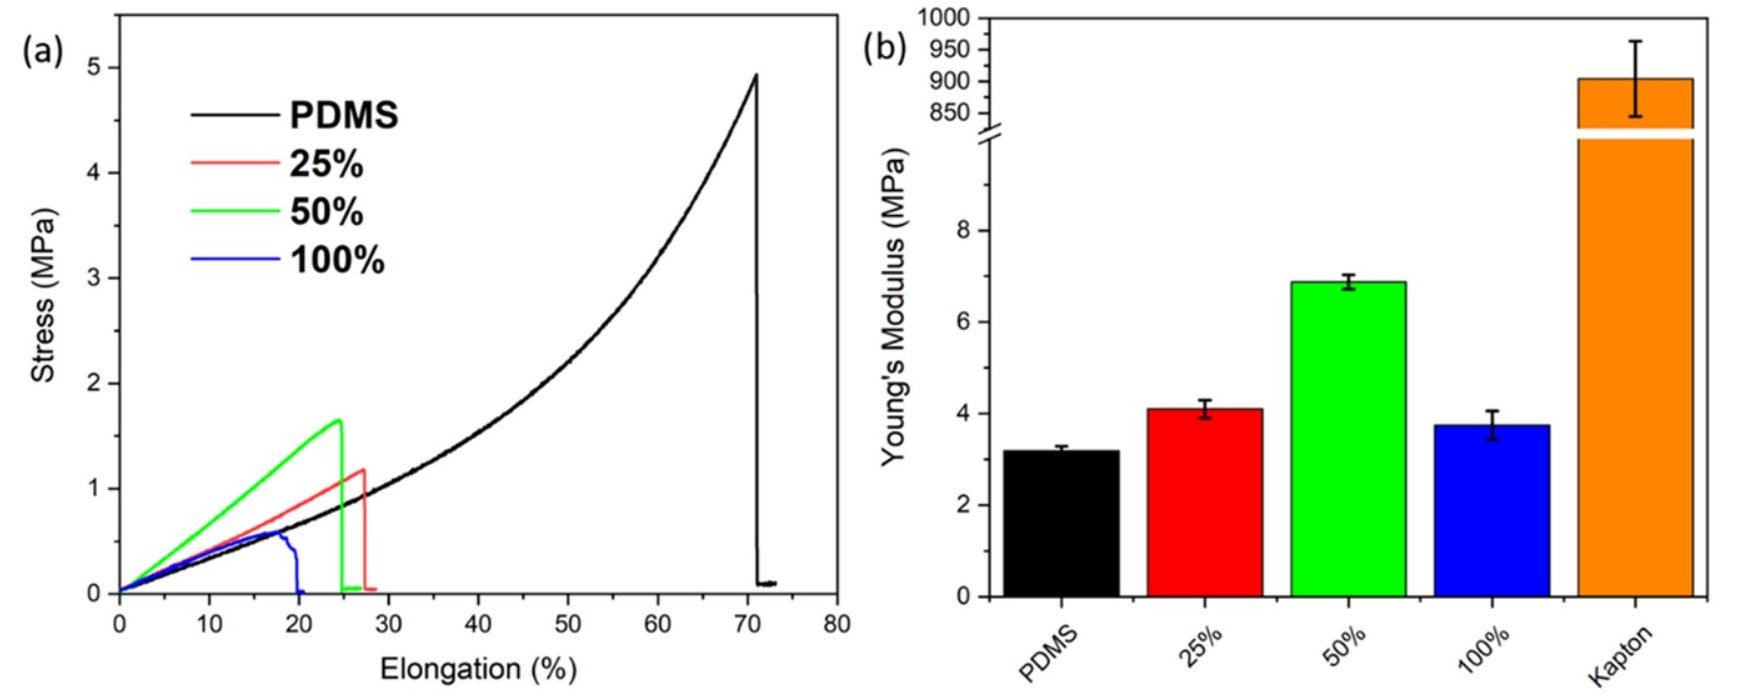
\includegraphics[width=1\textwidth]{Figures/Theory/PI_PDMS_Lamberti.jpg}
\medskip
\captionsetup{width=0.95\linewidth}
\caption{(a) Stress-strain curves up to the break point for the bare PDMS and the PDMS-PI composite. (b) Comparison of the Young's modulus of the bare PDMS, the PDMS-PI composite, and the Kapton. The reported values were obtained by averaging five different measurements for each
type of sample \cite{parmeggiani_pdmspolyimide_2019}.}
\label{fig:PI_PDMS_Lamberti}
\end{figure}

Using the described method authors fabricated supercapacitor devices of an interdigitated architecture with five pins per electrode as depicted in the inset of Figure \ref{fig:Lamberti_PDMS_PI_2019}.The cells were filled with 1 M $Na_2SO_4$ electrolyte solution and tested via cyclic voltammetry (CV), galvanostatic charge and discharge (CDG), and electrochemical impedance spectroscopy (EIS). The maximum resulting capacitance was estimated to be 25 $\mu F/cm^2$ for 1 $\mu A/cm^2$ current density during CDG experiment. 

\begin{figure}[H]
\centering
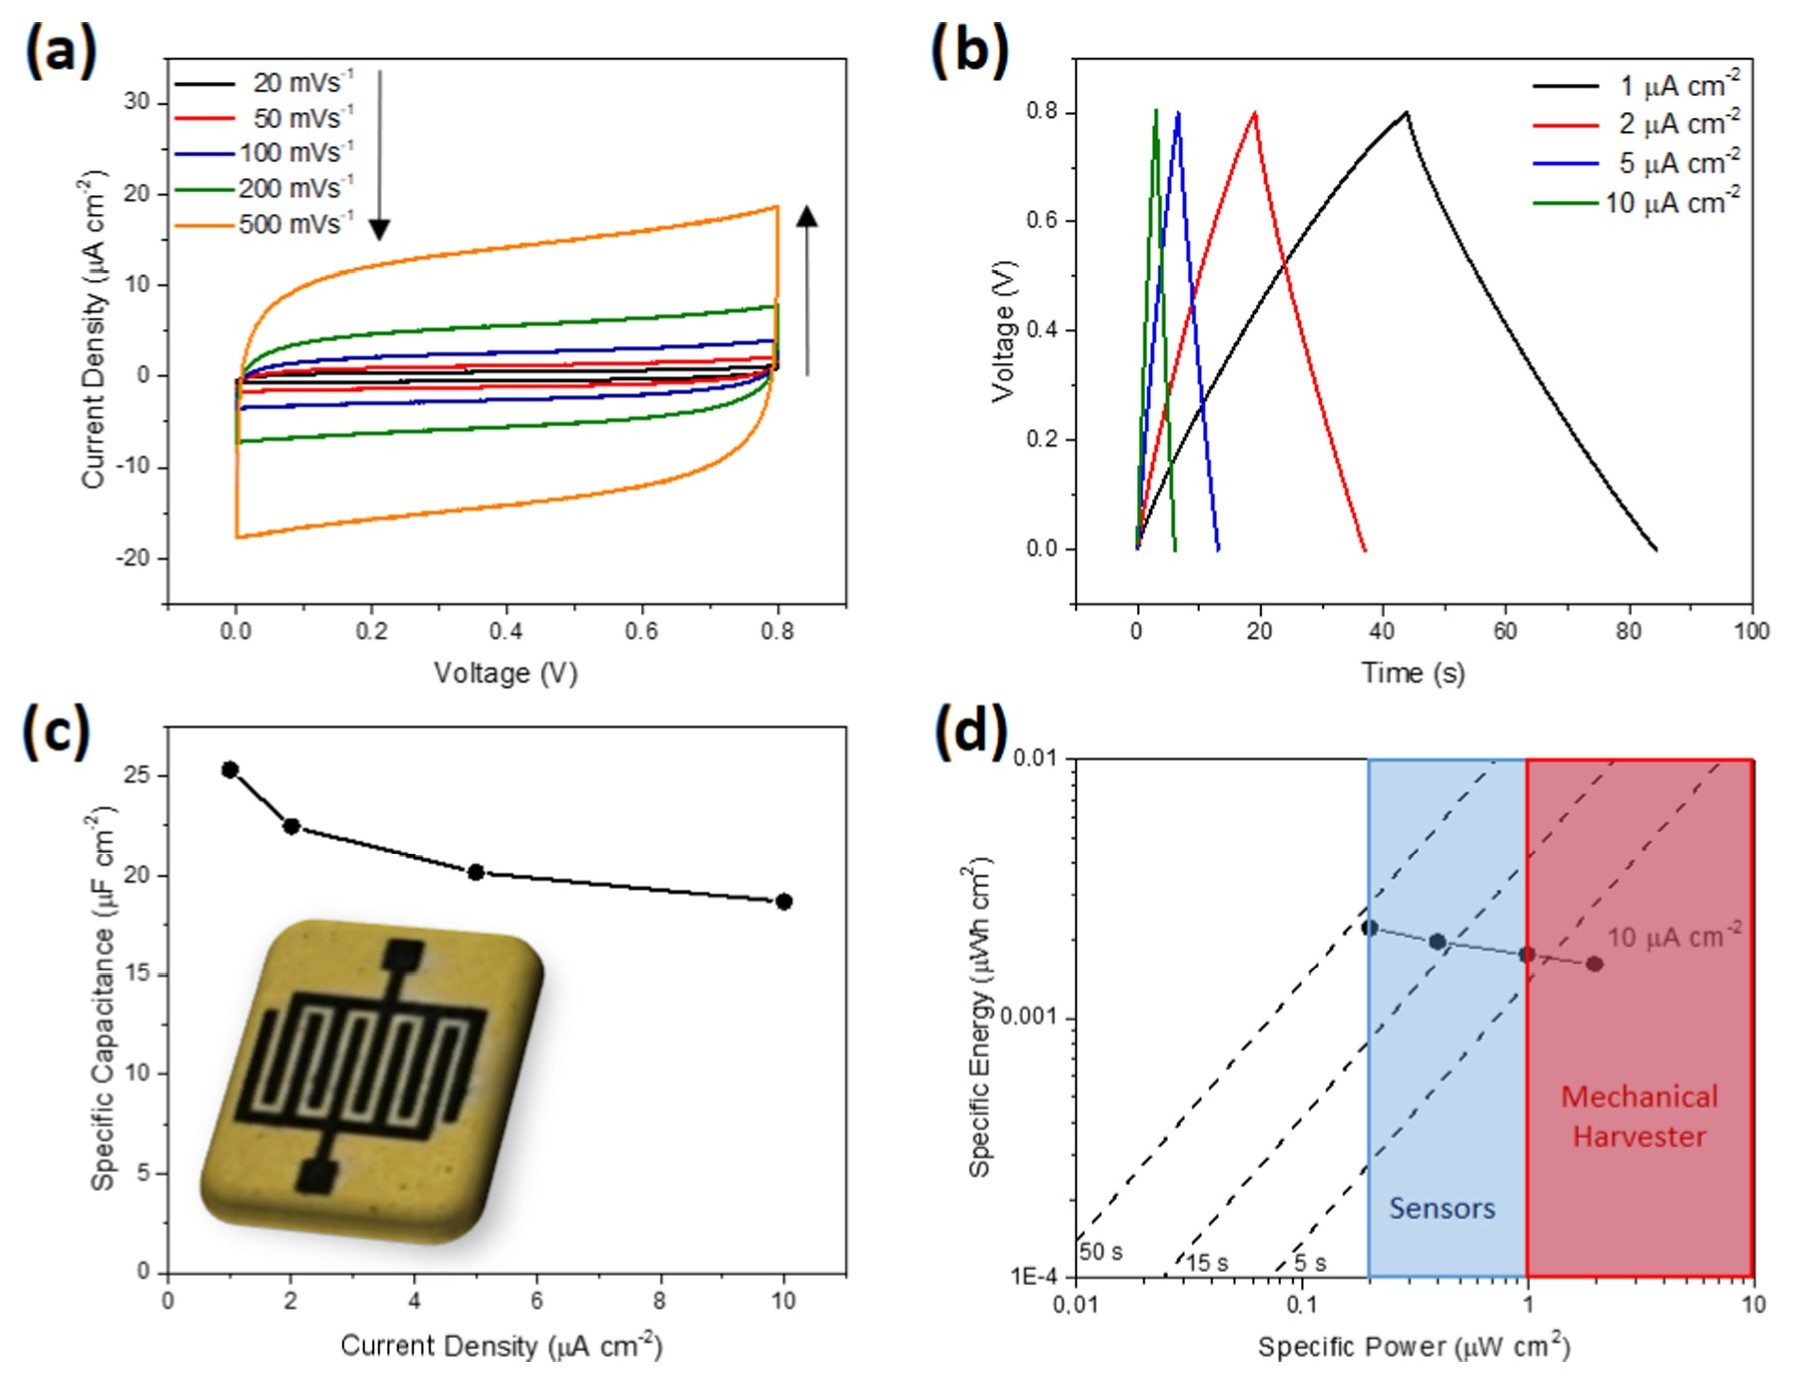
\includegraphics[width=1\textwidth]{Figures/Theory/Lamberti_PDMS_PI_2019.jpg}
\medskip
\captionsetup{width=0.95\linewidth}
\caption{Two-electrode electrochemical characterization of the SC in 1 M $Na_2SO_4$. (a) CV performed at several scan rates. (b) CDG performed at several current densities. (c) Cell capacitance and (d) Ragone plot derived from CDG tests \cite{parmeggiani_pdmspolyimide_2019}.}
\label{fig:Lamberti_PDMS_PI_2019}
\end{figure}

Recently \textbf{LAMPSe group \cite{dallinger_stretchable_2020}} has developed stretchable and ultrathin ($\approx$ 50 $\mu m$) skin-conformable conductors based on polyurethane covered with a conductive layer of LIG. Details of the fabrication procedure for this type of composite will be discussed in the Experimental Part \ref{chapter:Experimental set-up and Results}.  


\section{Materials Characterization Techniques}
\subsection{Surface Area and Porosity Characterization}

Surface area and porosity are two important physical properties that have a direct impact on the physical and chemical properties of materials. For a material used for electrochemical applications differences in the surface area and bulk pore size distribution can greatly influence its characteristics such as $e.g$ capacitance and power performance. These characteristics play the major role in electrochemical and other heterogeneous reactions taking place on the interfaces.

Before describing the gas adsorption analysis techniques the term porosity and associated to it nomenclature shall be defined. In the International Union of Pure and Applied Chemistry (IUPAC) defines porosity as "$A\;concept\;related\;to\;texture,\;referring\;to\;the\;pore\;space\;in\;a\;material.$" \cite{noauthor__1976}. Additionally the pore size definitions are introduced for those of three types: $the micropore$ width is defined as not to exceed about 2 nm, the mesopore width to be in the range 2–50 nm and the macropore width to be above about 50 nm \cite{SING19911}.

Gas Adsorption Analysis is the technique which is commonly used for surface area and porosity determinations. It involves exposing solid materials to gases at a variety of conditions and evaluating either the weight or the volume uptake by the solid sample. The latter is further referred to as the "adsorbent". These data allows to obtain information about the physical characteristics of the adsorbent, including: surface area $A$, skeletal density ($\mu_S$) - density of the material that constitute the particle, porosity, total pore volume (TPV), and pore size distribution.

Before the determination of an adsorption isotherms all of the physisorbed contaminants have to be removed from the surface of the adsorbent. At the same time the irreversible chemical as well as physical changes of the surface or the bulk structure should be avoided. This may be achieved by degassing, i.e., exposure of the surface to a high vacuum or an atmosphere. For non-microporous materials flushing the adsorbent with an inert gas (which may be the adsorptive) at elevated temperature is another technique which is often adopted. 

\medskip
\textbf{BET Surface Area Calculation}

Adsorption isotherms can be of different shapes and contain information about specific adsorption processes which take place on the investigated surfaces. The IUPAC classifies 6 types of the isotherms which are shown in Figure \ref{fig:isotherms_types}. 

\begin{figure}[H]
\centering
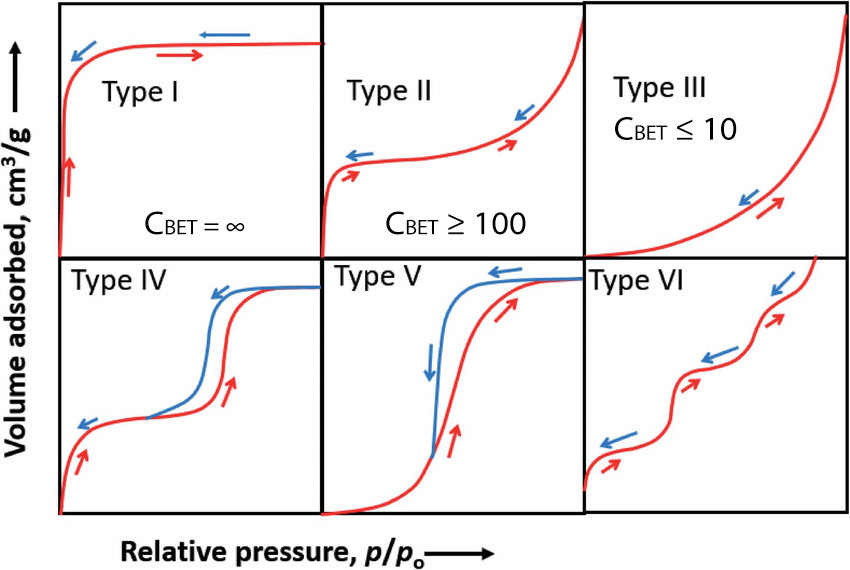
\includegraphics[width=0.6\textwidth]{Figures/Theory/isotherms_types.jpg}
\medskip
\caption{Different types of physisorption isotherms as observed for different adsorbents. Type I: microporous; Type II: non-porous or macroporous; Type III: non-porous or macroporous with weak interaction; Type IV: mesoporous; Type V: mesoporous with weak interaction; Type VI: layer-by-layer adsorption \cite{Kumar}}
\label{fig:isotherms_types}
\end{figure}

The Brunauer, Emmett and Teller (BET) technique invented in 1938 is the most common method for determining the surface area of powder and porous materials.  Nitrogen gas is usually used as the probe as it shows almost no chemosorption; the adsorbent under investigation is exposed to liquid nitrogen at low temperature conditions ($i.e.$ 77 K). The temperature of the solid sample is kept constant, or under isothermal conditions, while the pressure or concentration of the adsorbing gas is increased until it reaches a final pressure \(p^0\).
That allows to obtain information about gas adsorption as a function of pressure in a form of an isotherm graph, where the x-axis is the relative pressure of the gas and the y-axis is its volume adsorbed onto the sample. At first a BET plot is constructed for the relative pressure range \(0.05 \le p/p^0 \le 0.3\) for the mono-layer capacity $n_m$, mono-layer capacity, which is the volume of gas adsorbed at standard temperature and pressure (STP: 273 K and 1 atm), to be derived. The specific surface area $A_{BET}$ $[g/m^2]$ of the material is evaluated from the measured mono-layer adsorption capacity $n_m$ and knowledge of the cross-sectional area of the molecule being used as a probe, $\sigma$. The cross-sectional area of N$_2$ is taken as $\sigma$ =  16.2 $\si{\angstrom}^2$/molecule \cite{Kumar}. 
At each stage a certain level of assumptions is introduced into the evaluation procedure and thus it requires careful consideration for each investigated system.

The BET equation is conveniently expressed in the linear form with $p/p^0$ being partial pressure, $n$ specific volume of the gas adsorbed, $C$ an additional parameter limiting the number of layers on the surface \cite{noauthor_adsorption_nodate}, and $C_{BET}$ - BET constant dependent on the isotherm shape: 

\begin{equation}
\frac{p/p^0}{n(1-p/p^0)}=\frac{1}{n_mC} + \frac{C_{BET}-1}{n_mC_{BET}}\frac{p}{p^0}
  \label{eq:Bsp_BET_plot}
\end{equation}

Thus, the BET plot of \( \frac{p/p^0}{n(1-p/p^0)} \) versus \(p/p^0\) should be a straight line with slope \(s = \frac{C_{BET}- 1}{n_m C_{BET}} \) and intercept \( i = \frac{1}{n_m C_{BET}} \). By solving these two simultaneous equations, one obtains: 

\begin{equation}
    n_m = \frac{1}{s + i}
\end{equation}
and
\begin{equation}
    C_{BET} = \frac{s}{i} + 1
\end{equation}

The linear part of the isotherm is usually in the range  \(p/p^0 ~ 0.05-0.30 \) where the best linear fit is obtained by statistical analysis. Finally having $n_m$, $N_A$ - Avogadro Number and $m$ - adsorbent mass, the BET-area from the mono-layer capacity can be calculated as:

\begin{equation}
    A_{BET} = \frac{n_m \cdot N_A \cdot \sigma}{m}
\end{equation}

According to the Equation \ref{eq:Bsp_BET_plot} the values of $C_{BET}$  and \(p/p^0\) for a given $n_m$ is in a reciprocal dependency:
\begin{equation}
    \left(\frac{p}{p^0}\right)_{n_m}=\frac{1}{\sqrt{C_{BET}}+1}
\end{equation}

Which shows that high $C_{BET}$ values ($>350$) correspond to the low partial pressures and therefore to the high adsorption energy of the first layer and $vice\:versa$ when the adsorption energy and $C_{BET}$ values are low ($ < 20$) the partial pressures are high which might lead to an ill defined inflection point \cite{ROUQUEROL1999165} as can be seen from the exemplary isotherms in Figure \ref{fig:isotherms_types}. Type I and II of isotherms correspond to microporous solids and non-porous/macroporous,  respectively; the isotherm of Type III occurs for materials with high level of interactions between adsorbate and adsorbent. Another problem might arise from relatively weak adsorbent-adsorbate interactions together with comparatively strong adsorbate-adsorbate interactions, which is the case of the adsorption of water vapor on carbon materials.  For such systems, the BET mono-layer capacity is not reliable and does not provide a realistic assessment of total surface area magnitude if the surface was not properly prepared, $i.e.$ degassed and reduced in case of graphene oxide. However, it may provide a useful indication of the extent of the 'hydrophilic' area or the extent of the high-energy sites \cite{ROUQUEROL1999237}. 

\medskip
\textbf{Porosity Calculations}

The Barrett, Joyner, Halenda method (BJH) is commonly used for assessing the pore size distribution of mesoporous solids ($i.e.$ adsorbents having effective pore widths in the approximate range of 2-50 nm) and small macroporous materials ($i.e.$ with size range of 50-70 nm) . The model is based on the capillary condensation assumption in the $p/p^0$ region of 0.3 ± 1 and utilizes the Kelvin model of pore filling. The modified Kelvin equation \cite{ROUQUEROL1999165} relates the amount of adsorbate removed from the cylindrical pores of the material, as the relative pressure $p/p^0$ is decreased from a high to low value, to the size of the pores \ref{eq:Kelvin}. 

\begin{equation}
\label{eq:Kelvin}
    ln(\frac{p}{p^0})=\frac{2\gamma V_m}{RT(r_p - t_c)}
\end{equation}
Where: $V_m$ - liquid molar volume, $\gamma$ - surface tension of liquid nitrogen, $r_p$ - pore radius and $t_c$ - statistical thickness of the adsorbed multilayer film, which is formed prior to pore condensation.
The function of $t_c$ is given by an empirical function, one of which is called after Harkins and Jura and often used in BJH method. An in-depth description of this approach can be found in Chapter 7 in Rouquerol \textit{$et\:al.$}\cite{ROUQUEROL1999191}. 

For the micropores size distributions ($i.e.$ pores sizes $\le$ 2 nm) other theories are applied, among which the Non-local density functional theory (NLDFT) is one commonly used \cite{wu_jligorous_nodate}.

\subsection {Quantitative Morphological Characterization of Carbon Thin Films}
\label{Borghi-theory}

Although classical BET analysis is widely used and provides satisfactory results, it also has certain disadvantages, one of which is the demand for rather large amount of material for the typical experimental adsorption chambers. Another drawback of those chambers is the impossibility of studying the surface properties without distorting the original geometric configuration in which the material was obtained. This becomes especially important when working with films and other materials having a 2D shape. 

Just recently Francesca Borghi \textit{$et\:al.$} from University of Milan have invented a method for quantitative characterization of the interfacial morphology and bulk porosity of nanoporous cluster-assembled carbon thin films \cite{borghi_quantitative_2019}. In their work the authors utilize atomic force microscopy (AFM) and volumetric nitrogen adsorption technique for investigating the specific surface area, roughness and porosity of nanoporous carbon films. 

\medskip
\textbf{Morphological characterization}

The principle set-up of the AFM analysis of is explained in the following Figure \ref{fig:borghi_afm}.

\begin{figure}[H]
\centering
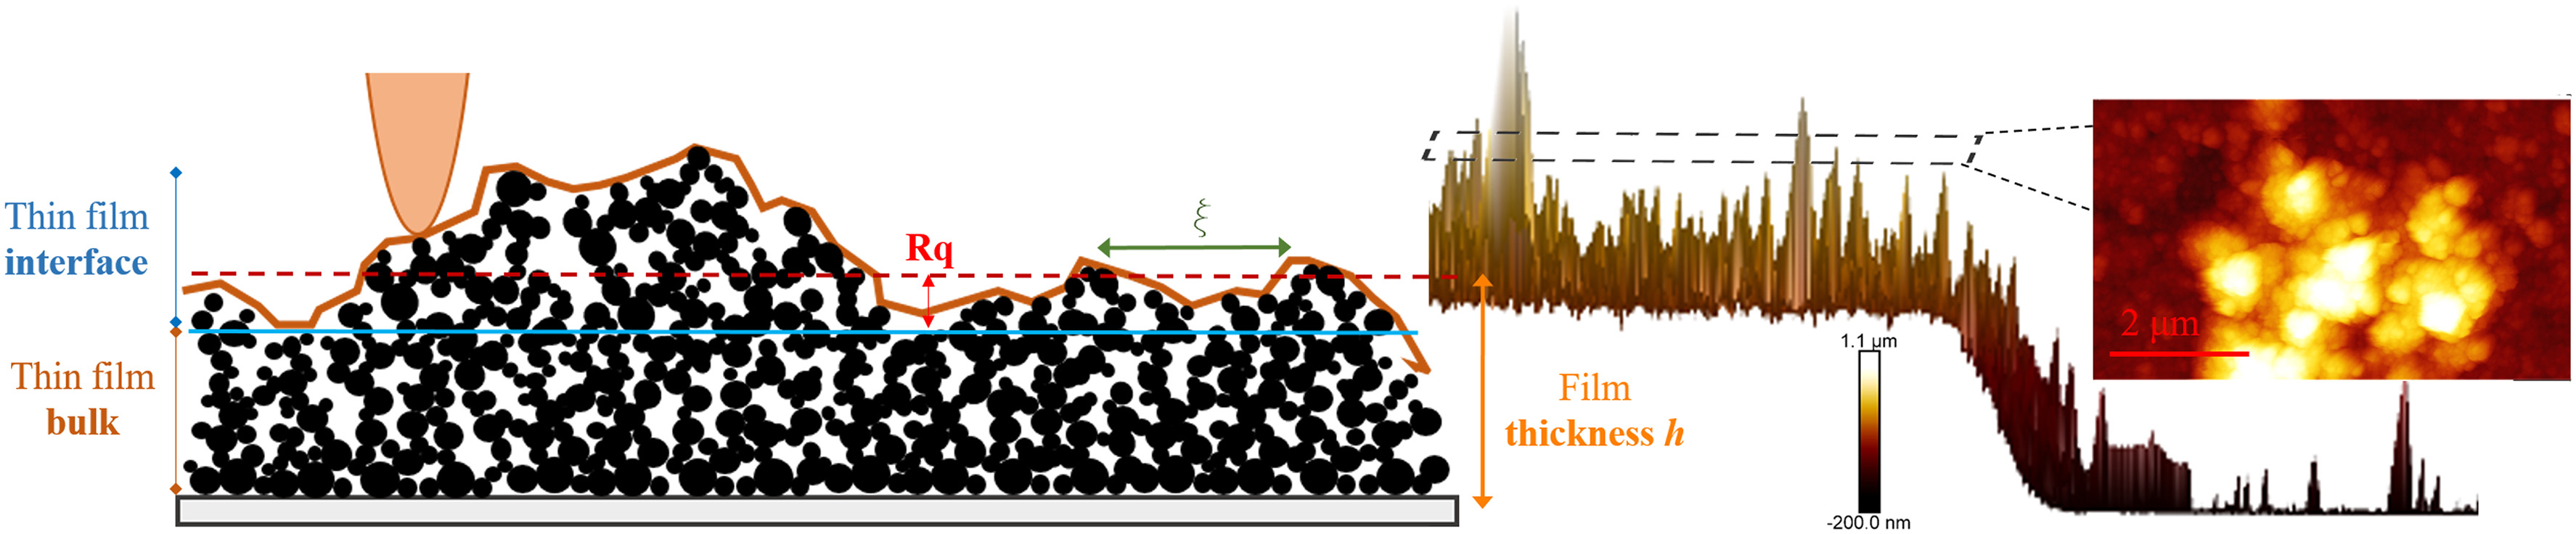
\includegraphics[width=1\textwidth]{Figures/Theory/AFM_Borghi.jpg}
\medskip
\caption{(Left) Representative schematic profile and morphological parameters of a nanoscaled-C thin film. (Right) 3D AFM view of a sharp step produced in an exemplary sample obtained on a Si substrate; in the inset, a representative topographic AFM map is shown (z scale ranges from -500 to 800 nm) \cite{borghi_quantitative_2019}}
\label{fig:borghi_afm}
\end{figure}

The images obtained by AFM were flattened by special mathematical technique, which allows to evaluate the morphological properties such as root-mean-square surface roughness $R_q$ (calculated as standard deviation of surface heights); the interfacial specific area $A_{spec}$ (calculated as the ratio of three-dimensional surface area scanned by AFM tip to the projected area); the correlation length $\xi$ representing the estimation of the halved lateral dimension of the biggest morphological features on the top of the surface. The latter can be equally seen as the aperture of the largest surface pores (see Figure \ref{fig:borghi_afm}). One of the most important characteristics, namely the film thickness $h$, was calculated as the mean distance between the film surface and the substrate. 

As mentioned earlier 2D shaped porous materials obtained on the surfaces can show different surface area values $in\:situ$ as compared to the bulk properties when investigated in the powder form. This fact can in turn drastically affect the effective surface area available for $e.g.$ heterogeneous reactions. The authors distinguish the top area by calling it thin film interface in order to highlight its possible morphological difference as compared to the thin film bulk which lays underneath. This approach becomes especially interesting when investigating the processes taking place on the top surface of the porous films as it allows to define the peculiarities of the interfacial area. 

\medskip
\textbf{Gas adsorption measurements}

For the gas adsorption measurements the samples of the thin carbon films obtained on silicone stripes 5 x 70 mm were at first degassed in helium atmosphere. The temperature dependence of degassing processes was carefully investigated and the best suitable conditions were found. Afterwards, the authors used a miniature experimental Gemini$^{TM}$ set-up which allowed to measure the bulk porosity of the thin carbon film samples without scribing the material from the surface. The advantage of this method lays in the fact it does not require large amounts of materials and the material itself can be put into a miniature gas tube chamber in the form it was prepared.  Obtained isotherms allowed to calculate the surface area and pores size distribution characteristics by applying BET and BJH methods respectively. In the described case of measurements the obtained $A_{BET}$ value represented the total surface area of both the thin film interface and bulk matrix, and was only limited by the diffusion and adsorption of nitrogen inside the carbon porous matrix on the surface of the substrate. 

\subsection{Mechanical Properties}

For materials characterization their electrical and mechanical behavior needs to be quantified. 

In regard to the \textbf{mechanical properties} typically a stress-strain curve, obtained in tensile, compression or shear experiments, is used. It shows the relation between a stress $\sigma$ [Pa] applied on a test coupon and a relative deformation caused by it. 


\begin{figure}[H]
\centering
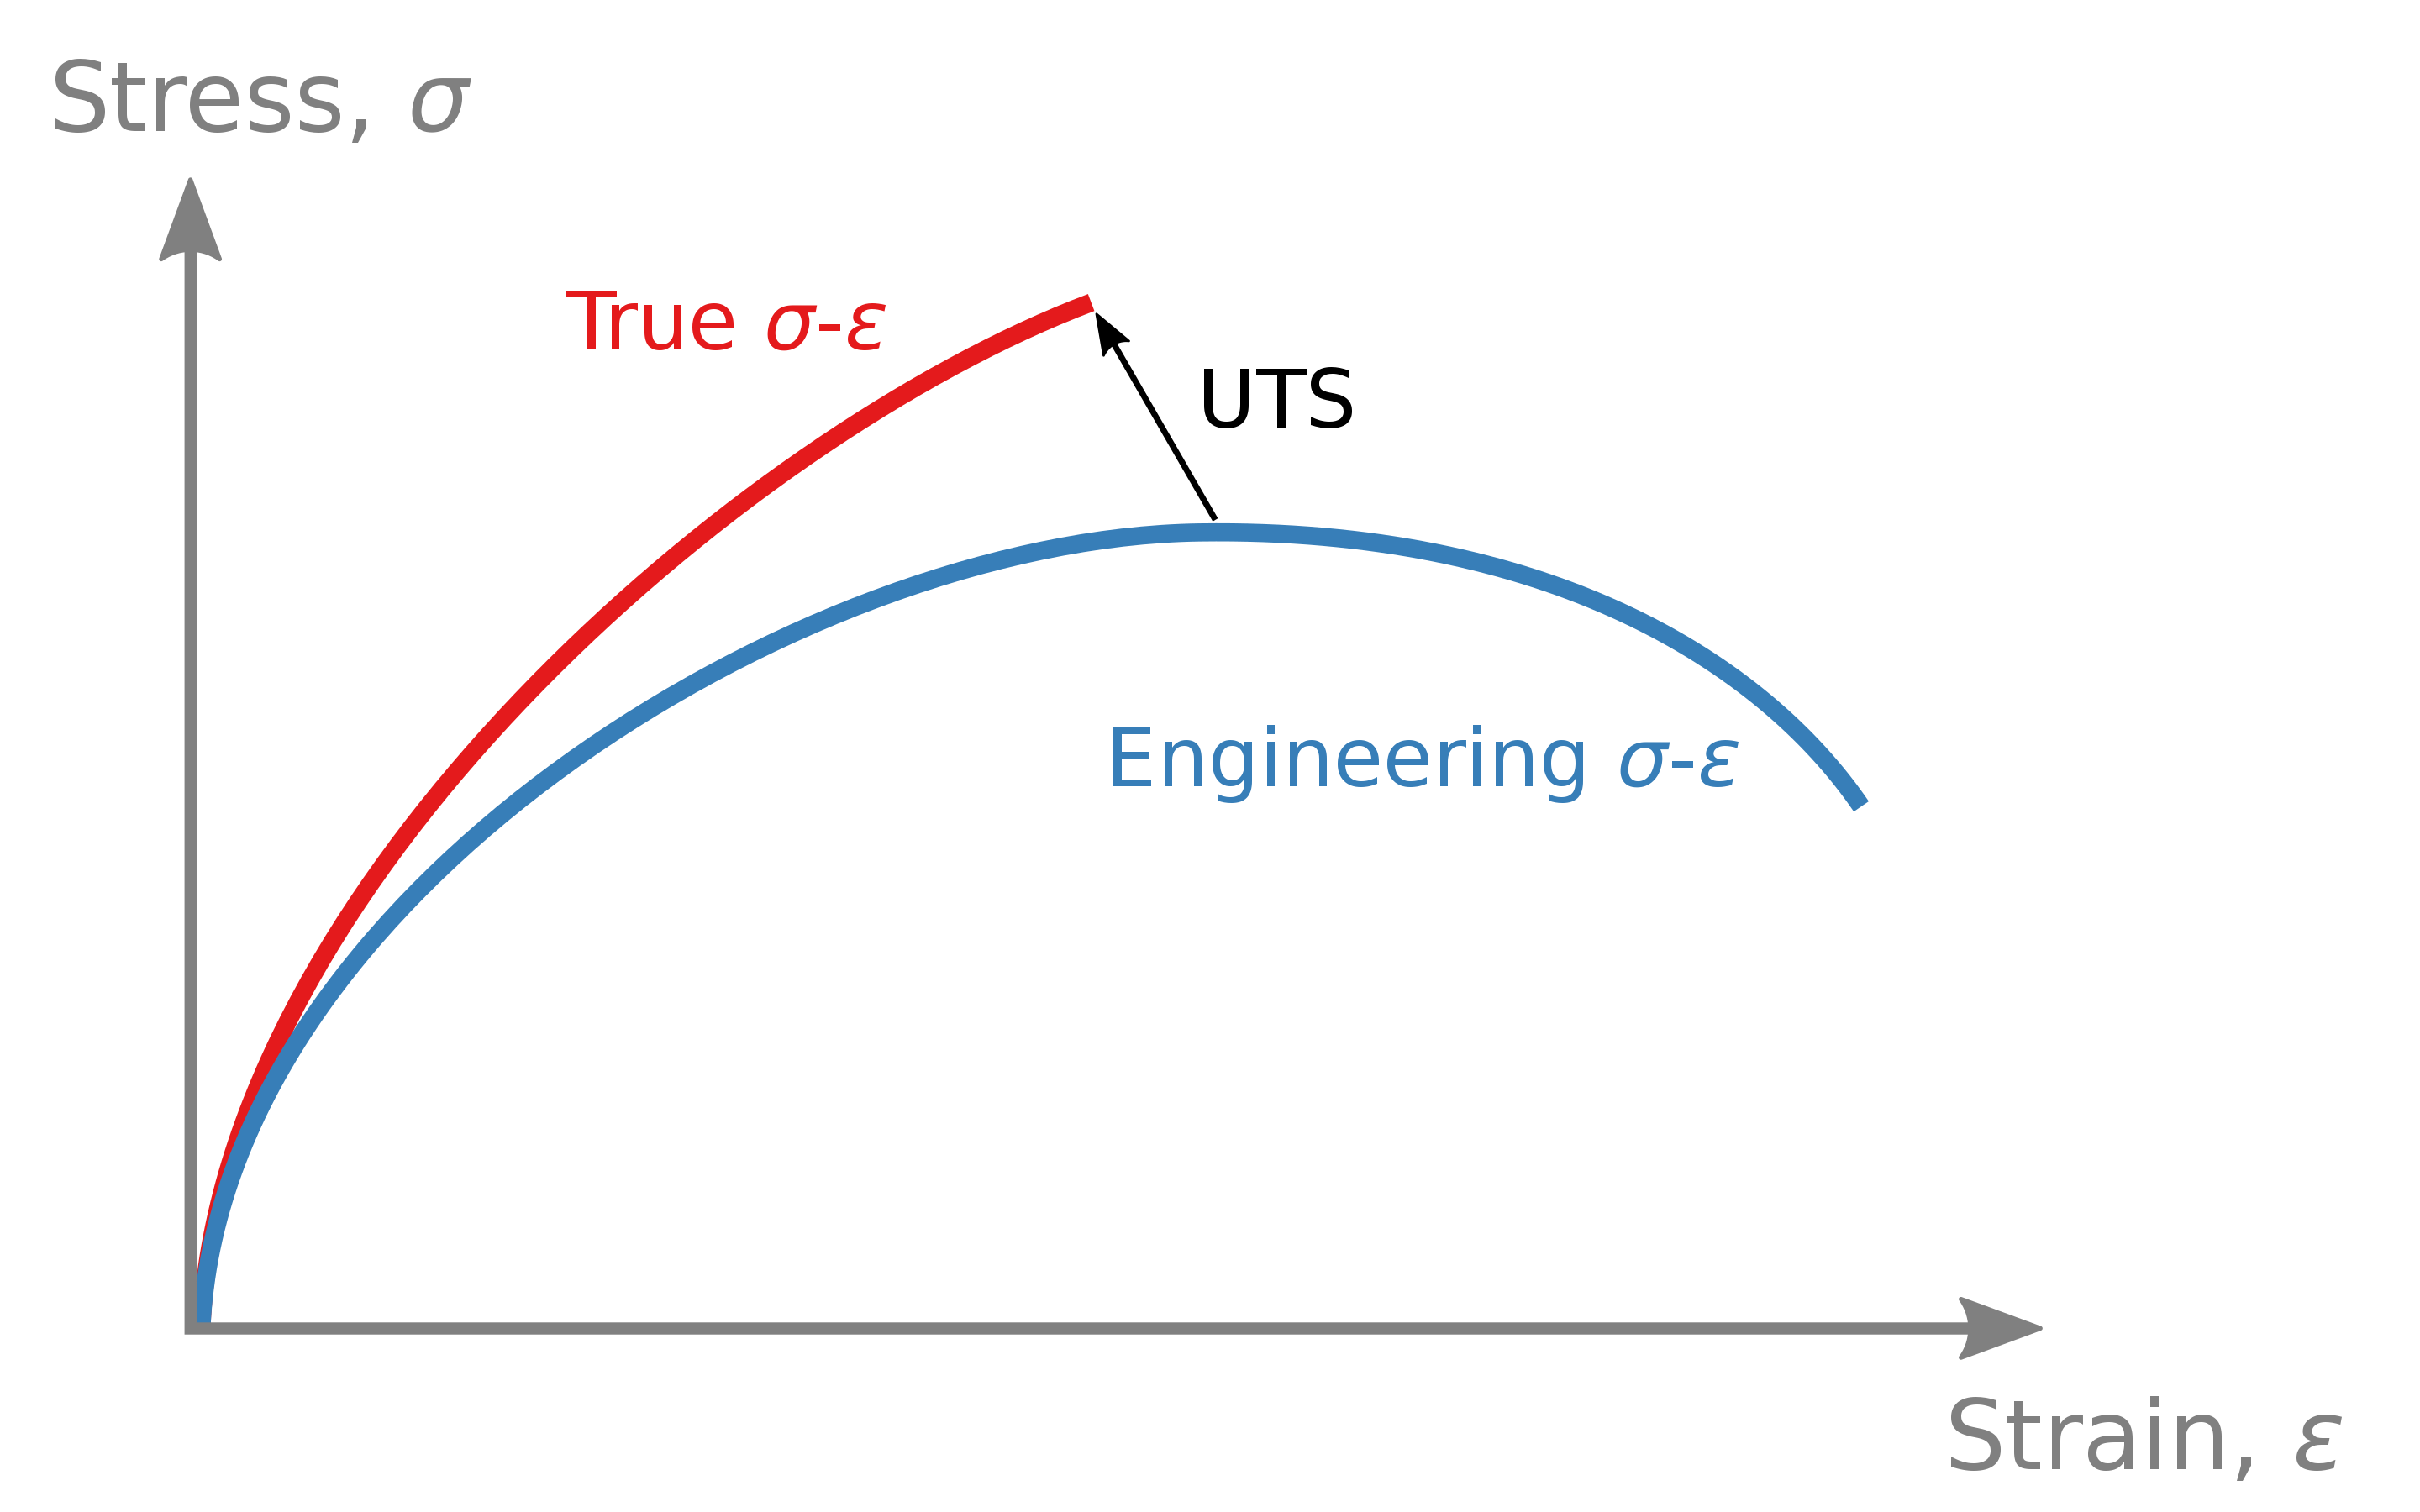
\includegraphics[width=0.6\textwidth]{Figures/Theory/2880px-Stress_strain_comparison.png}
\medskip
\captionsetup{width=0.6\linewidth}
\caption{The difference between true stress–strain curve and engineering stress–strain curve \cite{strain-stress-curve}.}
\label{fig:stress-curve}
\end{figure}

In many cases the deformation is appointed to elongation of a specimen and in general is called strain $\epsilon$ [a.u]:

\begin{equation}
\epsilon_t = \int \delta L/L
\label{eq:true_strain}
\end{equation}

Index $_t$ denotes the true elongation calculated for each further $\delta L$ in comparison to the developed elongation $\L$ at each moment of time during the experiment. In contrast engineering strain is calculated as:

\begin{equation}
\epsilon = L/L_0
\label{eq:strain}
\end{equation}

Where $L_0$ is the length of the specimen in the beginning. Engineering stress is therefore defined as:

\begin{equation}
\sigma = F/A_0
\label{eq:eng_stress}
\end{equation}

Where $F$ is the force applied, $A_0$ - specimen's cross section area at the beginning of the experiment. If the changes in the cross-section area are taken into account, then the stress curve is called $true\;stress$:

\begin{equation}
\sigma_t = F/A_t
\label{eq:true_stress}
\end{equation}

Equation connecting the engineering strain $\epsilon$ to the true strain $\epsilon_t$ is given by the formula:

\begin{equation}
\epsilon_t = \ln (L/L_0) = \ln (1+\epsilon)
\label{eq:true_strain_eng_strain}
\end{equation}

The graph of stress to strain allows to estimate yield strength, ultimate tensile strength (UTC), toughness as well as Young's modulus. The latter is calculated as a slope of a linear part of the curve, where the behavior is considered to be elastic:

\begin{equation}
E = \sigma / \epsilon
\label{eq:young}
\end{equation}

When undergoing deformation soft materials often exhibit viscoelastic properties showing time-dependent strain. Whereas elasticity is accounted to the stretching of bonds in an ordered solid, viscosity in turn is a consequence of the molecules aligning along the force vector and of the diffusion of atoms in an amorphous material \cite{meyers2008mechanical}. 


\subsection{Electrical Properties}

One of the important characteristics of a material is its electrical conductivity $\sigma$ or its inverse value - electrical resistivity $\rho$. For thin films it is common to calculate these parameters by measuring sheet resistance $R_s$ [$\Ohm / sq$]  of a flat sample of a known thickness $\theta$ by a four-probe method: 

\begin{equation}
\sigma = \frac{1}{\rho} = \frac{1}{R_s \times \theta} 
\label{eq:conductivity}
\end{equation}

A four-probe method makes use of a four equally-spaced, co-linear probes which are brought in an electrical contact with the material. The main advantage of this method is the elimination of contact and wire resistance $i.e$ inner resistance components of the measurement setup from the final result. A diagram of the measurement setup is shown in Figure \ref{fig:four-probe} below. 

During the measurement a DC current $I$ is applied between the outer probes, whereas a voltage drop $\Delta V$ is measured between the inner two probes. 

\begin{figure}[H]
\centering
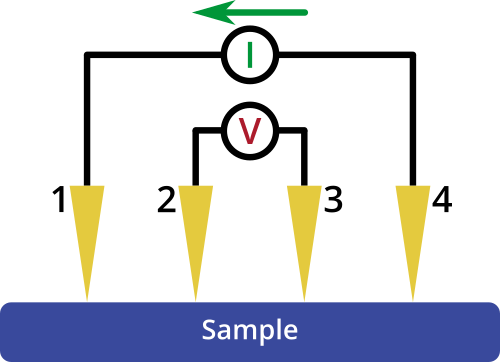
\includegraphics[width=0.5\textwidth]{Figures/Theory/four-point-probe-circuit-schematic.png}
\medskip
\captionsetup{width=0.8\linewidth}
\caption{Schematic diagram of a four-point probe circuit \cite{ossila}.}
\label{fig:four-probe}
\end{figure}

Following equation is used to calculate $R_s$:
\begin{equation}
R_s = \frac{\pi}{\ln (2)}\frac{\Delta V}{I} 
\label{eq:sheet-res}
\end{equation}

The geometric correction factor $\frac{\pi}{\ln (2)}$ is required to take the shape of the sample, as well as the positioning of the probes into account. The most accurate results are obtained for probing the center of the sample \cite{ossila}. Equation \ref{eq:sheet-res} only applies when the sample's size significantly larger, 40 and more times greater, than the spacing of the probes. The thickness $\theta$ has to be less than 40\% of the probe spacing. Smaller sample dimensions might limit the current paths between the probes which results in a overestimated values of $R_s$. In this case, an additional correction factor $C_f$ accounting for the specified geometry of the sample is introduced \cite{geometr-resistivity}, \cite{geometr-resistivity-corr}:

\begin{equation}
R_s = \frac{\pi}{\ln (2)}\frac{\Delta V}{I}C_f 
\label{eq:sheet-res-corr}
\end{equation}



%This fact has to be taken into account when setting the experiment to explore $e.g$ \textbf{electrical properties} of such materials.


\subsection{Swelling, Viscoelastic, Electrical Properties in Wet Conditions}

\section{Supercapacitors}
Intro, what it is.

\subsection{Electrochemical Characterization of Cells}

\textbf{Cyclic Voltammetry}

\textbf{Galvanostatic Cycling with Potential Limitation}

\textbf{Impedance spectroscopy}


% \section{(Wettability of composite surfaces)}
